%
%
\chapter{Eletromagnetísmo}


\begin{enumerate}[start=1,label={\bfseries Q\arabic*.}]



\item Um solenoide muito longo, de seção reta circular de raio $R$, com $n$ voltas por unidade de comprimento, tem uma corrente elétrica dada por $I(t) = I_{0} \sin \omega t$. Seu eixo encontra-se ao longo do eixo $z$ de um sistema de coordenadas. Assuma o limite quase-estático ($\omega R << c$) e que o campo magnético \textbf{B} fora do solenoide é nulo.

a) Calcule o vetor campo magnético \textbf{B} dentro do solenoide.

\resposta

Por simetria, $\mathbf{B} = B\hat{z}$. A lei de Ampère é válida no limite quase-estático. Aplicando-a a um circuito retangular com dois lados paralelos de comprimento $L$ na direção $z$, sendo um dentro do solenoide e outro fora, e os dois outros lados na direção radial,

$$
\oint \mathbf{B} \cdot \mathrm{d} \mathbf{l}=B_{z} L=\mu_{0} I(S)=\mu_{0} n L I(t) \Rightarrow \mathbf{B}=\mu_{0} n I_{0} \sin (\omega t) \hat{\mathbf{z}} \quad(r<R)
$$

onde I(S) é a corrente total que atravessa o circuito e usamos que a contribuição dos lados radiais do circuito para a circulação de B é nula (porque $\mathbf{B}  \bot  dl$) e o campo magnético é nulo fora do solenoide.


b) Calcule o vetor campo elétrico \textbf{E} dentro do solenoide.

\resposta

Usando a lei de indução de Faraday

$$
\oint \mathbf{E} \cdot \mathrm{d} \mathbf{l}=-\frac{\mathrm{d}}{\mathrm{d} t} \iint \mathbf{B} \cdot \hat{\mathbf{n}} \mathrm{d} \mathbf{S}
$$

aplicada a um circuito circular de raio $r < R$, com eixo ao longo de $z$ e concêntrico ao solenoide ($\hat{n} = \hat{z}$) e usando que, por simetria, o campo elétrico é azimutal $\mathbf{E} = E\hat{\theta}$

$$
E 2 \pi r=-\pi r^{2} \frac{\mathrm{d}}{\mathrm{d} t} B, \Rightarrow \mathrm{E}(\mathrm{r})=-\frac{1}{2} \mu_{0} n \omega I_{0} r \cos (\omega t) \hat{\theta} \quad(r<R)
$$



c) Calcule o vetor campo elétrico \textbf{E} fora do solenoide.

Procedendo de maneira análoga ao item anterior mas agora com $r > R$

$$
E 2 \pi r=-\pi R^{2} \frac{\mathrm{d}}{\mathrm{d} t} B, \Rightarrow \mathrm{E}(\mathrm{r})=-\frac{1}{2 r} \mu_{0} n \omega I_{0} R^{2} \cos (\omega t) \hat{\theta} \quad(r>R)
$$

\resposta

Procedendo de maneira análoga ao item anterior mas agora com $r > R$

$$
E 2 \pi r=-\pi R^{2} \frac{\mathrm{d}}{\mathrm{d} t} B, \Rightarrow \mathrm{E}(\mathrm{r})=-\frac{1}{2 r} \mu_{0} n \omega I_{0} R^{2} \cos (\omega t) \hat{\theta} \quad(r>R)
$$








\item Um circuito RC é composto de um resistor de resistência $R$ ligado em série a um capacitor de capacitância $C$. No instante $t = 0$, uma bateria de voltagem $V$ é conectada ao circuito. O capacitor, inicialmente descarregado, consiste em duas placas metálicas circulares de raio $a$ separadas por uma distância $d$ (d << a) e com vácuo entre elas. Despreze efeitos de borda no capacitor, ou seja, considere o campo elétrico uniforme entre as placas e nulo fora delas. Assuma o limite quase-estático.



a) Calcule a capacitância $C$ do capacitor.

\resposta

A densidade superficial de carga $\sigma$ na placa com carga total $Q$ é relacionada ao campo elétrico $E$ entre as placas por $\sigma = Q/ \pi a^{2}) = \epsilon_{0} E$. A diferença de potencial entre as placas $U$ é relacionada ao campo elétrico por $E = U / d$. Como, por definição, $Q = CU$, segue que

$$
C=\frac{\epsilon_{0} \pi a^{2}}{d}.
$$



b) Calcule a corrente elétrica no circuito como função do tempo para $t > 0$.

\resposta

Pela lei de Kirchhoff

$$
V=R I+\frac{Q}{C}=R \frac{\mathrm{d} \mathrm{Q}}{\mathrm{d} t}+\frac{Q}{C}
$$

A solução dessa equação diferencial que satisfaz a condição inicial $Q(0) = 0$ é

$$
Q=V C\left(1-e^{-t / \tau}\right), \operatorname{com} \tau=R C
$$

Segue que,

$$
I=\frac{\mathrm{d}}{\mathrm{d} t} Q=\frac{V}{R} e^{-t / \tau}.
$$


c) Calcule o vetor campo magnético \textbf{B} nas bordas laterais da regi˜ao entre as placas do capacitor como função do tempo para $t > 0$.

\resposta

Como a carga (e o campo elétrico) no capacitor muda(m), campo magnético é gerado. Aplicaremos a lei de Ampère-Maxwell

$$
\oint \mathbf{B} \cdot \mathrm{d} \mathbf{l}=\mu_{0} \int \mathbf{J} \cdot \hat{\mathbf{n}} \mathrm{d} S+\mu_{0} \epsilon_{0} \frac{\mathrm{d}}{\mathrm{d} t} \int \mathbf{E} \cdot \hat{\mathbf{n}} \mathrm{d} S
$$

a um circuito circular de raio $a$ paralelo às placas do capacitor, a meio caminho entre elas e com centro no seu eixo. Nesse caso, $\mathbf{J} = 0$ e $\hat{\mathbf{n}} || \mathbf{E} = \frac{\sigma}{\epsilon_{0}} \hat{z}$. Além disso, $\mathbf{B} = B\hat{\theta}$ (por simetria). Segue que

\begin{eqnarray*}
B 2 \pi a &=& \mu_{0} \epsilon_{0} \frac{\mathrm{d}}{\mathrm{d} t} \int E \mathrm{d} S=\mu_{0} \epsilon_{0} \frac{\mathrm{d}}{\mathrm{d} t} \int \frac{Q(t)}{\epsilon_{0} \pi a^{2}} \mathrm{d} S=\mu_{0} \frac{\mathrm{d}}{\mathrm{d} t} Q(t)=\mu_{0} I(t) \\
&\Rightarrow & \quad \mathrm{B}=\frac{\mu_{0} I(t)}{2 \pi a} \hat{\theta}
\end{eqnarray*}



d) Calcule o vetor de Poynting e a taxa temporal de energia eletromagnética entrando na regi˜ao entre as placas do capacitor enquanto ele é carregado.

\resposta

O vetor de Poynting na borda do capacitor é

$$
\mathrm{S}=\frac{1}{\mu_{0}} \mathbf{E} \times \mathbf{B}=\frac{Q(t)}{\epsilon_{0} \pi a^{2}} \hat{\mathbf{z}} \times \frac{I(t)}{2 \pi a} \hat{\boldsymbol{\theta}}, \Rightarrow \mathbf{S}=-\frac{Q I}{\epsilon_{0} 2 \pi^{2} a^{3}} \hat{\mathbf{r}}
$$

A taxa temporal de energia eletromagnética que flui para dentro do capacitor é a integral do módulo do vetor de Poynting na sua área lateral

$$
P=S 2 \pi a d=\frac{Q I d}{\epsilon_{0} \pi a^{2}}=I E d=I U
$$
onde, como antes, U é a diferença de potencial entre as placas.







\item Um disco de raio $a$ feito de um material isolante gira em torno do seu eixo de simetria com velocidade angular $\omega$ constante. Uma espira de cobre, na forma de um setor circular de ângulo $\pi/4$ e mesmo raio $a$, está presa à superfície do disco como mostra a figura abaixo. A resistência elétrica da espira é $R$. Um campo magnético externo de módulo $B$, perpendicular ao disco e entrando no plano da figura, está presente na região do espaço delimitada pelos ângulos fixos $\theta = \pi/4$ e $\theta = 3 \pi/4$.

\begin{figure}[H]
\centering
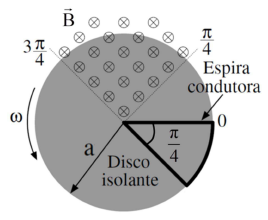
\includegraphics[scale=0.8]{eletromag-img/espira}
\end{figure}



a) Calcule o módulo da corrente elétrica induzida na espira quando esta entra ou sai da região de campo magnético.

\resposta

b) Convencionando como positiva a corrente que circula na espira no sentido horário, faça o gráfico da corrente induzida como função do tempo para o intervalo de tempo de uma de uma revolução do disco. Considere como instante inicial aquele ilustrado na figura.

\resposta

c) Calcule a energia total dissipada na espira em um ciclo.

\resposta

d) Calcule o torque da força magnética sobre a espira, com relação ao centro do disco, quando ela entra na região de campo magnético. Além do módulo, determine a direção e o sentido do \textbf{vetor} torque.

\resposta




\item Uma esfera condutora maciça de raio $R$ está carregada e imersa simetricamente entre dois dielétricos de permissividades elétricas $\textepsilon_{1}$ e $\textepsilon_{2}$, conforme ilustrado na figura abaixo. Resolvendo-se a equação de Laplace, pode-se mostrar que o potencial eletrostático fora da esfera ($r > R$) é dado por $V(\vec{r}) = A/r$, sendo $A$ uma constante e $r = |\vec{r}|$. Expresse as suas respostas em termos de $A$, $R$, $\textepsilon_{1}$, $\textepsilon_{2}$, e da posição $\vec{r}$.

\begin{figure}[H]
\centering
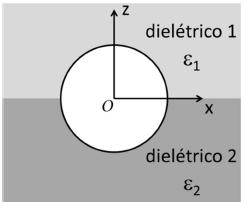
\includegraphics[scale=1]{eletromag-img/dieletrico}
\end{figure}


a) Calcule o potencial eletrostático $V(\vec{r})$ e o campo elétrico $\vec{E}(\vec{r})$ no interior da esfera ($r < R$).

\resposta

b) Calcule o campo elétrico $\vec{E}(\vec{r})$ e o deslocamento elétrico $\vec{D}(\vec{r})$ fora da esfera ($r > R$), em cada dielétrico (dielétrico 1 e dielétrico 2).

\resposta

c) Quais são as densidades superficiais de carga livre na superfície da esfera condutora adjacente a cada um dos dielétricos?

\resposta

d) Há carga de polarização na interface entre os dois dielétricos? Se sim, quanto vale a densidade superficial dessa carga? Se não, justifique.

\resposta




\item Um capacitor de placas paralelas condutoras tem suas duas placas perpendiculares à direção $z$. Uma das placas, localizada em $z = 0$, tem um potencial elétrico $V = 0$, enquanto a outra placa, localizada em $z = d$, tem um potencial elétrico $V = V_{0}$, onde $V_{0}$ é uma constante. No espaço entre as placas, preenchido por um dielétrico com permissividade elétrica $\epsilon$, a densidade de carga elétrico livre é dada por
$$
\rho_{F}(z) = \rho_{0} e^{-\alpha z},
$$
onde $\rho_{0}$ e $\alpha$ são constantes. Despreze os efeitos de borda.



a) Mostre que o potencial entre as placas é da forma
$$
V(z) = A + Bz - \frac{\rho_{0}}{\epsilon \alpha^{2}} e^{\alpha z},
$$
onde $A$ e $B$ são constantes.

\resposta O problema se resume a resolver a equação de Poisson
$$
\nabla^{2} V = - \frac{\rho}{\epsilon}
$$
No nosso caso a simetria do problema dita que $V (\vec{r}) = V (z)$. Portanto,
$$
\nabla^{2} V = \frac{d^{2} V}{dz^{2}} = - \frac{\rho}{\epsilon} e^{-\alpha z}.
$$
Integrando a Eq. (8) uma vez em z teremos
$$
\frac{dV}{dz} = B + \frac{\rho_{0}}{\epsilon \alpha} e^{-\alpha z}.
$$
Integrando agora a Eq. (9) uma vez em $z$ teremos finalmente
$$
V(z) = A + Bz + \frac{\rho_{0}}{\epsilon \alpha} e^{-\alpha z}
$$
onde $A$ e $B$ são constantes de integração.



b) Determine as constantes $A$ e $B$ a partir das condições de contorno.

\resposta Impondo as condições de contorno,
$$
V(z=0) = 0 \Rightarrow 0 = A - \frac{\rho_{0}}{\epsilon \alpha^{2}} \Rightarrow A = \frac{\rho_{0}}{\epsilon \alpha^{2}}.
$$
$$
V(z=d)=V_{0} \Rightarrow V_{0}=A+B d-\frac{\rho_{0}}{\epsilon \alpha^{2}} e^{-\alpha d} \Rightarrow B=\frac{1}{d}\left[V_{0}+\frac{\rho_{0}}{\epsilon \alpha^{2}}\left(e^{-\alpha d}-1\right)\right].
$$

c) Determine o \textbf{vetor} campo elétrico entre as placas.

\resposta Do item (b), o potencial é dado por

$$
V(z)=\frac{\rho_{0}}{\epsilon \alpha^{2}}+\frac{1}{d}\left[V_{0}+\frac{\rho_{0}}{\epsilon \alpha^{2}}\left(e^{-\alpha d}-1\right)\right] z-\frac{\rho_{0}}{\epsilon \alpha^{2}} e^{-\alpha z}
$$
Temos que
$$
\mathrm{E}=-\nabla V=-\frac{\partial V}{\partial x} \hat{\mathrm{x}}-\frac{\partial V}{\partial y} \hat{\mathrm{y}}-\frac{\partial V}{\partial z} \hat{\mathrm{z}}=-\frac{d V}{d z} \hat{\mathrm{z}}
$$
Portanto
$$
\begin{aligned}
\mathbf{E} &=-\left\{\frac{1}{d}\left[V_{0}-\frac{\rho_{0}}{\epsilon \alpha^{2}}\left(1-e^{-\alpha d}\right)\right]+\frac{\rho_{0}}{\epsilon \alpha^{2}} \alpha e^{-\alpha z}\right\} \hat{\mathbf{z}} \\
&=\frac{1}{d}\left[\frac{\rho_{0}}{\epsilon \alpha^{2}}\left(1-e^{-\alpha d}-\alpha d e^{-\alpha z}\right)-V_{0}\right] \hat{\mathbf{z}}
\end{aligned}
$$








\item a) Um segmento retilíneo de fio, de comprimento $L$, transporta uma corrente $i$. Calcule o módulo do campo magnético $B$, produzido pelo segmento no ponto $P$, localizado a uma distância $R$ do segmento e equidistante de suas extremidades, como mostra a Figura (a).
\begin{figure}[H]
\centering
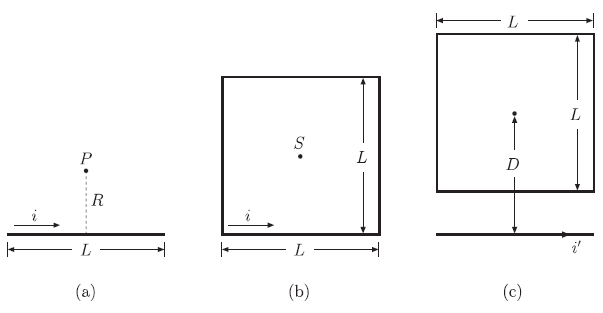
\includegraphics[scale=1]{eletromag-img/aros.png}
\end{figure}

\resposta A lei de Biot-Savart é

$$
\mathbf{B}(\mathbf{r})=\frac{\mu_{0} i}{4 \pi} \int_{C} \frac{d \mathbf{l}^{\prime} \times\left(\mathbf{r}-\mathbf{r}^{\prime}\right)}{\left|\mathbf{r}-\mathbf{r}^{\prime}\right|^{3}}
$$
Tomando um sistema de referência tal que $d \mathrm{l}^{\prime}=d x^{\prime} \hat{\mathrm{x}}, \mathrm{r}^{\prime}=x^{\prime} \hat{\mathrm{x}}$ e $\mathrm{r}=R \hat{\mathrm{y}}$
$$
\mathbf{B}(P)=\frac{\mu_{0} i}{4 \pi} \int_{-L / 2}^{L / 2} \frac{R d x^{\prime} \hat{\mathbf{z}}}{\left(R^{2}+x^{\prime 2}\right)^{3 / 2}}=\frac{\mu_{0} i R}{2 \pi} \int_{0}^{L / 2} \frac{d x^{\prime}}{\left(R^{2}+x^{2}\right)^{3 / 2}} \hat{\mathbf{z}}
$$
Usando a integral fornecida no formulário
$$
\mathbf{B}(P)=\frac{\mu_{0} i}{2 \pi R} \frac{L}{\sqrt{4 R^{2}+L^{2}}} \hat{\mathbf{z}}
$$
Portanto,
$$
B(P)=\frac{\mu_{0} i}{2 \pi R} \frac{L}{\sqrt{4 R^{2}+L^{2}}}
$$



b) Use o resultado do item (a) e obtenha $B$ quando $R << L$. Compare o resultado com o módulo do campo magnético gerado por um fio muito longo.

\resposta A Eq. (10) no limite $R << L$ torna-se
$$
B = \frac{\mu_{0} i}{2 \pi R}.
$$
Este é o módulo do campo magnético gerado por um fio infinito, como obtido facilmente pela aplicação direta da lei de Ampère.


c) Considere agora uma espira quadrada de fio, de lado $L$, transportando uma corrente $i$, como na Figura (b). Calcule o módulo do campo magnético $B$ no ponto $S$, localizado no centro da espira.

\resposta A espira quadrada é formada pela junção de 4 segmentos de fio de comprimento $L$. Como as contribuições de cada segmento são vetorialmente idênticas, o campo no centro da espira será simplesmente a soma das contribuições individuais de cada segmento. O módulo resultante é, portanto,
$$
 B = \left.4 \frac{\mu_{0} i}{2 \pi R} \frac{L}{\sqrt{4 R^{2}+L^{2}}}\right|_{R=L / 2}=\frac{2 \sqrt{2} \mu_{0} i}{\pi L}
$$


d) Uma espira quadrada de fio, de lado $L$ e sem nenhuma corrente, é colocada próxima a um fio infinitamente longo que transporta uma corrente $i'$. A distância do fio longo ao centro da espira é $D$, como mostrado na Figura (c). Determine a intensidade do fluxo magnético gerado pelo fio através da espira.

\resposta O campo magnético gerado por um fio longo infinito, transportando uma corrente $i'$, em uma distância $r'$ do fio, é dado por
$$
\mathbf{B}=\frac{\mu_{0} i^{\prime}}{2 \pi r^{\prime}} \hat{z}
$$
O fluxo de campo magnético $\Phi_{B}$ através da superfície da espira é dado por
$$
\Phi_{B}=\int_{S} \mathbf{B} \cdot \hat{n} d a
$$
onde $d a=d x d y$ e $\hat{n}=\hat{\mathbf{z}},$ logo
$$
\mathbf{B} \cdot \hat{n}=\frac{\mu_{0} i^{\prime}}{2 \pi r^{\prime}}=\frac{\mu_{0} i^{\prime}}{2 \pi y}
$$
Portanto,
$$
\Phi_{B}=\int_{S} \frac{\mu_{0} i^{\prime}}{2 \pi y} d x d y=\frac{\mu_{0} i^{\prime}}{2 \pi} \int_{-L / 2}^{L / 2} d x \int_{D-L / 2}^{D+L / 2} \frac{d y}{y}=\frac{\mu_{0} i^{\prime}}{2 \pi} L \ln \left(\frac{2 D+L}{2 D-L}\right)
$$





\item Um espectrômetro de massa simples pode ser construído como esquematizado na figura. Um feixe de íons positivos de massa $m$ e carga $q$  (linha pontilhada) sai de uma fonte $S$, é acelerado pela diferença de potencial elétrico $V$ e penetra por uma fenda de entrada numa câmara onde há um campo magnético uniforme $B$ saindo perpendicularmente do plano do papel. Após percorrer uma trajetória semicircular de raio $r$, o feixe sai pela fenda de saída e é detectado por um deterctor $D$ se a massa for compatível com a trajetória. Dessa forma, é possível selecionar íons pelo valor de sua massa, ajustando o valor de $B$. As fendas de entrada e de saída da câmara são iguais. Todo o sistema está em vácuo. Despreze a interação gravitacional do feixe.

\begin{figure}[H]
\centering
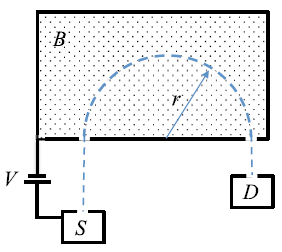
\includegraphics[scale=1]{eletromag-img/espec.png}
\end{figure}




a) Determine o módulo da velocidade dos íons ao passarem pela fenda de saída em termo de $V$, $m$ e $q$.

\resposta

b) Determine $m$ em função de $V$, $B$, $r$ e $q$.

\resposta

c)A resolução das medidas de massa do aparelho é limitada pelo tamanho da fenda de saída,que determina o erro do raio $r$. Considere uma situação em que $r = 10 cm$, $V = 4,0 \times 10^{3} \mbox{V}$, $B = 1,00 \mbox{T}$ e que cada íon tem um elétron a menos que o átomo neutro correspondente. Se as fendas têm tamanho $100 \ \mu m$, qual é a resolução das medidas de massa?

\resposta

d) É possível usar esse aparelho para distinguir os isótopos de carbono $^{12}\mbox{C}$ de $^{14}\mbox{C}$? Justifique.

\resposta




\item Considere a propagação de ondas eletromagnéticas num meio linear, homogêneo e istrópico com condutividade elétrica $\sigma$, permissividade elétrica $\epsilon$ e permeabilidade magnética $\mu$, na ausência de fontes de cargas elétricas livres ($\rho_{F} = 0$).


a) Escreva as equações de Maxwell para os campos elétrico $\mathbf{E}$ e magnético $\mathbf{B}$ no meio, em termos de $\sigma$, $\epsilon$ e $\mu$.

\resposta

b) Encontre a equação diferencial que envolve apenas o campo elétrico $\mathbf{E}$.

\resposta

c) Considere uma solução do tipo onda plana $\mathbf{E}(x,t) = \mathbf{E}_{0} e^{i(kx - \omega t)}$ e obtenha a relação entre $k$ e $\omega$ em termos de $\sigma$, $\epsilon$ e $\mu$.

\resposta

d) Com relação ao resultado do item (c), interprete fisicamente a diferença entre os casos $\sigma \neq 0$ e $\sigma = 0$.

\resposta




\item Considere o circuito representado na figura. Inicialmente, o capacitor está descarregado. No instante $t=0$ a chave $S_{1}$ é fechada.

\begin{figure}[H]
\centering
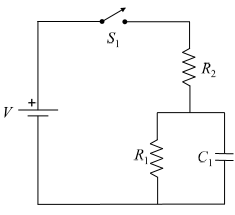
\includegraphics[scale=1]{eletromag-img/quadrada.png}
\end{figure}


a) Quais são os valores da corrente que passa pelo resistor de resistência $R_{1}$ em $t = 0$ e após um longo tempo?

\resposta

b) Qual é a carga no capacitor de capacitância $C_{l}$ após um longo tempo?

\resposta

c) Faça três gráficos esquemáticos das diferenças de potencial como funções do tempo entre as extremidades dos resistores de resistências $R_{1}$ e $R_{2}$ e do capacitor de capacitância $C_{1}$ a partir de $t = 0$, indicando claramente os valores máximos e mínimos.

\resposta

d) Depois de permanecer ligada por um longo tempo, a chave $S_{1}$ é desligada em $t = t_{d}$. Quanto tempo então decorre para que a carga do capacitor caia para uma fração $l/e$ do seu valor em $t = t_{d}$? ($e \approx 2.718$ é a base dos logaritmos naturais)

\resposta





\item Um guia de ondas muito usado em laboratórios é o cabo coaxial. Ele consiste de um fio condutor interno rodeado por um isolante (branco) dentro de uma malha condutora, protegida por um encapamento isolante (preto), como mostrado na foto da esquerda. Ele pode ser modelado como um fio metálico interno de raio a dentro de um dielétrico com permissividade elétrica 6 e permeabilidade magnética p e uma casca metálica cilíndrica de raio interno b, como indicado na figura da direita. A corrente percorre o fio interno numa direção e a casca cilíndrica na direcão contrária.

\begin{figure}[H]
\centering
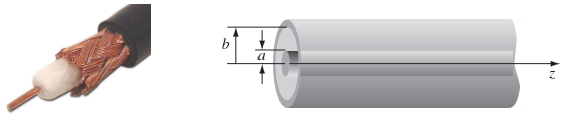
\includegraphics[scale=1]{eletromag-img/coaxial.png}
\end{figure}


\item(a) Use a simetria do problema e a lei de Gauss para obter a capacitância por unidade de comprimento do cabo em termos de e, V, a e b.

\resposta

\item(b) Use a simetria do problema e a lei de Ampàre para obter a auto-indutância por unidade de comprimento do cabo em termos de e, V, a e b. Dica: calcule a energia armazenada no campo magnético em um comprimento finito do cabo e iguale o resultado a LI 2/2, onde L é a auto-indutância e I é a corrente pelo cabo.

\resposta





\item Um anel fino de raio $R$ e carga total $Q > 0$ uniformemente distribuída ao longo de sua circunferência está fixo no plano $xy$ de um sistema de coordenadas e tem seu centro na origem $O$. Seja $P$ um ponto com coordenadas $(0,0,z)$ (ver figura abaixo).
\begin{figure}[H]
\centering
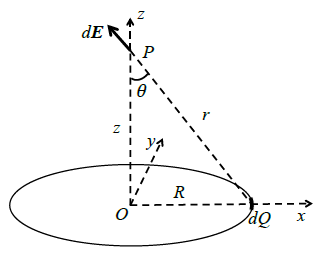
\includegraphics[scale=1]{eletromag-img/anel.png}
\end{figure}

a) Somando as contribuições de todos os elementos de carga do anel, encontre módulo, direção e sentido do campo elétrico $\vec{E}(z)$ no ponto $P$.

\resposta O elemento de carga $d Q$ do anel produzirá um campo $d \vec{E}$ no ponto $P$, como mostrado na figura. O mádulo deste elemento de campo elétrico é
$$
d E = \frac{d Q}{4 \pi \epsilon_{0} r^{2}}.
$$
\begin{figure}[H]
  \centering
  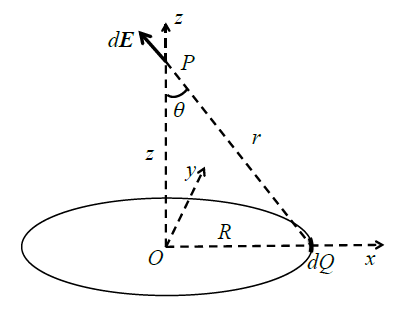
\includegraphics[scale=0.7]{eletromag-img/anel3.png}
  %\caption{}\label{}
\end{figure}
A componente deste elemento de campo elétrico perpendicular ao eixo $z$ é cancelada pela componente perpendicular ao eixo $z$ produzida pelo elemento de carga situado na posição diametralmente oposta do anel. Ao somar os elementos de campo elétrico devido a todos os elementos de carga do anel, apenas sobrevivem as componentes na direção do eixo $z$
$$
d E_{z}=\frac{d Q}{4 \pi \epsilon_{0} \tau^{2}} \cos \theta=\frac{d Q}{4 \pi \epsilon_{0} r^{2}} \frac{z}{r}
$$
Somando todas as contribuições dos elementos de carga do anel, obtemos
$$
\vec{E}=\hat{z} \frac{Q z}{4 \pi \epsilon_{0} r^{3}}=\hat{z} \frac{Q z}{4 \pi \epsilon_{0}\left(R^{2}+z^{2}\right)^{3 / 2}}
$$


b) Proceda analogamente ao item (a) e calcule o potencial elétrico $V (z)$ no ponto $P$.

\resposta O potencial elétrico devido ao elemento de carga $d Q$ no ponto $P é$
$$
d V(z)=\frac{d Q}{4 \pi \epsilon_{0} r}
$$
O potencial devido a todas as contribuições dos elementos de carga do anel é obtido somando todas as contribuições, donde se obtém
$$
V(z)=\frac{Q}{4 \pi \epsilon_{0} r}=\frac{Q}{4 \pi \epsilon_{0} \sqrt{R^{2}+z^{2}}}
$$


c) Uma partícula pontual de carga $- q < 0$ e massa $m$ parte do repouso de um ponto com coordenadas $(0,0,z_{0})$, muito distante da origem (ou seja, $z_{0} >> R$) e viaja ao longo do eixo $z$. Qual é a sua velocidade quando ela passa pelo centro do anel? Considere desprezíveis os efeitos da radiação eletromagnética emitida pela partícula no seu trajeto em direção ao centro do anel.

\resposta A energia cinética inicial da partícula é nula, porque ela parte do repouso. A energia potencial elétrica inicial da partícula é nula também, porque $-q V\left(z_{0}\right) \approx 0$ se $z_{0} \gg R$. A conservação da energia mecânica (cinética mais potencial elétrica) nos dá a velocidade $v$ no centro do anel via
$$
0+0=\frac{m v^{2}}{2}+(-q) V(0)=\frac{m v^{2}}{2}-q \frac{Q}{4 \pi \epsilon_{0} R}
$$
donde
$$
v=\sqrt{\frac{q Q}{2 \pi \epsilon_{0} m R}}
$$





\item Um aro quadrado rígido de arame com lado $L$ tem resistência elétrica total $R$. O aro está no plano $xy$ de um sistema de coordenadas e move-se com velocidade $\vec{v}$ para fora da regi˜ao onde há um campo magnético uniforme $\vec{B}$ (area sombreada na figura abaixo) apontando para fora da página (sentido de $z$ positivo). Considere o instante em que o vértice da esquerda do aro está a uma distância $s$ dentro da area sombreada ($0 < s < \sqrt{2}L/2$).

\begin{figure}[H]
\centering
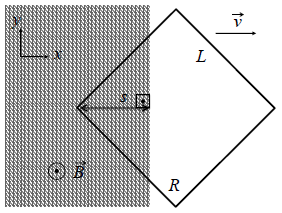
\includegraphics[scale=1]{eletromag-img/aro.png}
\end{figure}


a) Calcule o fluxo do campo magnético através do aro como função de $s$.

\resposta Como o aro $\hat{\epsilon}$ quadrado, a área da região interna ao aro e contida no retângulo sombreado
é um triângulo isósceles de altura $s$ e ângulos internos $45^{\circ}, 90^{\circ}$ e $45^{\circ} .$ Portanto, o tamanho da base do triângulo é 2 s e sua área é
$$
A=\frac{1}{2} s(2 s)=s^{2}
$$
O fluxo do campo magnético através do aro é
$$
\Phi=\int \vec{B} \cdot d \vec{S}=B A=B s^{2}
$$
onde usamos o fato de que o campo magnético $B$ constante na região sombreada e normal ao plano da figura.
\begin{figure}[H]
  \centering
  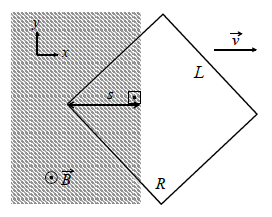
\includegraphics[scale=0.7]{eletromag-img/aro3}
 % \caption{}\label{}
\end{figure}



b) Determine o valor e o sentido de circulação da corrente elétrica induzida no aro.

\resposta b) A força eletromotriz induzida pode ser calculada pela lei de Faraday:
$$
\varepsilon=-\frac{d \Phi}{\partial t}=-B 2 s \frac{d s}{d t}=-2 B s v
$$
e o valor da corrente elétrica é
$$
I=\frac{2 B s v}{R}
$$
A área sombreada diminui com o movimento do aro e, portanto, o fluxo do campo magnético também diminui. O sentido da força eletromotriz, pela lei de Lenz, é anti-horário para se contrapor à diminuição do fluxo de $\bar{B}$. Segue que a corrente fluirá também no sentido anti horário.

c) Calcule a força magnética total (módulo, direção e sentido) sobre o aro quando a corrente induzida circula nele. Que força adicional à força magnética deve ser aplicada no aro para que ele se mova com velocidade constante sob a ação exclusiva dessas duas forças?

\resposta A força magnética sobre um elemento do aro é
$$
d \vec{F}_{m}=I d \vec{l} \times \vec{B}
$$
Os elementos do aro dentro da região sombreada são: $d \vec{l}=-\frac{\sqrt{2}}{2}(\hat{x} d l+\hat{y} d l)$ (lado superior esquerdo) e $d \vec{l}=\frac{\sqrt{2}}{2}(\hat{x} d l-\hat{y} d l)$ (lado inferior esquerdo). A força magnética é, então,
$$
d \vec{F}_{m}=I\left[-\frac{\sqrt{2}}{2}(\hat{x} d l+\hat{y} d l) \times B \hat{z}+\frac{\sqrt{2}}{2}(\hat{x} d l-\hat{y} d l) \times B \hat{z}\right]
$$
ou
$$
d \vec{F}_{m}=-\sqrt{2} I B d l \hat{x}
$$
e integrando em $d l$ de 0 a $\sqrt{2} s$ (lembrando que as contribuições dos dois segmentos já foram somadas) obtemos
$$
\vec{F}_{m}=-2 I B s \hat{x}
$$
Substituindo a Eq. (5) na Eq. (6), obtemos
$$
\vec{F}_{m}=-\hat{x} \frac{4 B^{2} s^{2} v}{R}
$$
Para que o quadrado se mova com velocidade constante, temos que aplicar uma força de mesmo módulo que $\vec{F}_{m},$ mas de sentido oposto, isto é para a direita (sentido positivo de $x$ ).






\item Dois aros circulares finos encontram-se no plano $xy$ de um sistema de coordenadas, ambos com centro na origem. Um aro tem raio $b$ e uma densidade linear de carga elétrica $-\lambda < 0$ e o outro tem raio $2b$ e uma densidade linear de carga elétrica $2 \lambda > 0$.


a) Calcule o potencial eletrostático $V (z)$ no ponto $P = (0,0,z)$.

\resposta

b) Calcule o vetor campo elétrico $\vec{E}(z)$ no ponto $P = (0,0,z)$.

\resposta

c) Escreva a equação da segunda lei de Newton para uma partícula de carga $q > 0$ e massa $m$, restrita a se mover ao longo do eixo $z$ e sujeita ao campo elétrico do item (b). Além da força elétrica, nenhuma outra força atua sobre a partícula.

\resposta

d) Calcule a frequência de pequenas oscilações para a partícula do item (c) na vizinhança de $z = 0$. Dica: linearize a força em torno de $z = 0$.




\item Uma onda eletromagnética plana monocromática que se propaga no vácuo com polarização circular é descrita, em notação complexa, pelo campo elétrico $\tilde{\mathbf{E}}(\mathbf{r},t) = E_{0}e^{i(kz-\omega t)} \left(\hat{X} + i \hat{Y} \right)$, onde $\omega = ck$ é a frequência angular, $c$ é a velocidade da luz no vácuo, $k$ é o número de onda, $E_{0}$ é uma amplitude real e $i = \sqrt{-1}$.


a) Encontre o campo elétrico real (físico) $\mathbf{E}(\mathbf{r},t)$.

\resposta

b) Encontre o campo magnético real (físico) $\mathbf{B}(\mathbf{r},t)$ usando as equações de Maxwell. Se preferir, utilize $\nabla \rightarrow ik$.

\resposta

c) Calcule a densidade de momento linear da onda eletromagnética $g = \epsilon_{0} \mathbf{E} \times \mathbf{B}$.

\resposta

d) Calcule a densidade de momento angular da onda eletromagnética $\mathbf{l} = \mathbf{r} \times \mathbf{g}$. Dica: use coordenadas cilíndricas $r = \rho \hat{\rho} + z \hat{z}$.



\item Definindo-se o vetor de Hertz $\vec{Z}$ pelas expressões:
\begin{equation}
\vec{\nabla} \cdot \vec{Z} = -\phi; \quad \vec{A} = \mu_{0} \epsilon_{0} \frac{\partial \vec{Z}}{\partial t},
\end{equation}

onde $\phi$ e $\vec{A}$ são, respectivamente, os potenciais escalar e vetor.


a) Mostre que os potenciais satisfazem o calibre de Lorentz:

\begin{equation}
\vec{\nabla} \cdot \vec{A} + \mu_{0} \epsilon_{0} \frac{\partial \phi}{\partial t} = 0;
\end{equation}

\resposta

b) Demonstre que para um meio sem fontes ($\rho = 0$, $\vec{J} = 0$) e de $\mu = \mu_{0}$ o vetor $\vec{Z}$ satisfaz às seguintes expressões:

\begin{equation}
\nabla^{2} \vec{Z} - \frac{1}{c^{2}} \frac{\partial^{2} \vec{Z}}{\partial t^{2}} = - \frac{\vec{P}}{\epsilon_{0}}; \quad
\vec{B} = \frac{1}{c^{2}} \vec{\nabla} \times \frac{\partial \vec{Z}}{\partial t}; \quad \vec{E} = \vec{\nabla} \times \vec{\nabla} \times \vec{Z} - \frac{\vec{P}}{\epsilon_{0}},
\end{equation}
onde $\vec{P}$ é o vetor de polarização.

\resposta

\item Considere um disco vazado muito fino, com raio interno $r_{1}$ e raio externo $r_{2}$, deitado sobre o plano $xy$ e com o eixo centrado em $z = 0$ (conforme ilustrado na figura 1).

\begin{figure}[H]
\centering
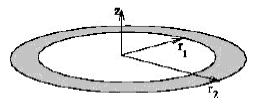
\includegraphics[scale=1]{eletromag-img/vasado.png}
\end{figure}

O anel tem densidade superficial de carga dada por:
\begin{equation}
\sigma (r) = \frac{\sigma_{0}}{r}
\end{equation}

onde $r  = \sqrt{x^{2} + y^{2}}$


a) Encontre o campo elétrico $\vec{E}(x = y = 0, z$) sobre o eixo $z$;

\resposta

b) Suponha agora que o anel comece a girar com velocidade angular $\omega_{0}$. Encontre a densidade de corrente $\vec{J}_{s} = \sigma \vec{v}$, onde $\vec{v}$ é a velocidade linear;

\resposta

c) Encontre o campo magnético $\vec{H}(x = y = 0;z)$ sobre o eixo $z$, gerado pela densidade de corrente $\vec{J}_{s}$.




\item Uma esfera isolante sólida de raio $a$ tem densidade de carga uniforme $\rho$ carga total $Q$. Uma esfera oca condutora não carregada, cujos raios interno e externo são $b$ e $c$, respectivamente, é concêntrica à esfera isolante, como mostra a figura abaixo.

\begin{figure}[H]
\centering
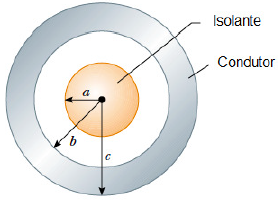
\includegraphics[scale=1]{eletromag-img/esfera.png}
\end{figure}


a) Determine a magnitude do campo elétrico nas regiões: $(i) \ r < a; \ (ii) \ a < r < b; \ (iii) \ b < r < c \ e \ (iv) \ r > c$.

\resposta Pela lei de Gauss, de maneira geral, sabemos que:
%
\begin{equation} \label{eq9}
  \oint \vec{E} \cdot d \vec{S} = \frac{q_{V}}{\epsilon_{o}}
\end{equation}
%
onde a integral é feita sobre a superfície $S$ de uma região $V$ e $q_{V}$ é a carga total contida em $V$. Tomaremos, nessa questão, regiões esféricas de raio $r$ centradas no centro da esfera isolante. Por simetria, o campo elétrico apontará sempre na direção radial, ou seja, $\vec{E} = E \hat{r}$.

i) Campo elétrico para $r < a$: Neste sub-item, escolhemos regiões esféricas de raio $r < a$, representadas pelas linhas pontilhadas na Fig. \ref{imagenspng}. Desta forma, a carga em $V$ é
%

\begin{equation}
  \begin{array}{ccc}
    q_{V} & = & \rho V \\
    q_{V} & = & \frac{4 \pi \rho}{3} r^{3} .
  \end{array}
\end{equation}
%

Aplicando a Eq. (\ref{eq9}) e usando que o campo elétrico é radial
\begin{equation}
  E 4 \pi r^{2} = \frac{4 \pi \rho}{3 \epsilon_{o}} r^{3} .
\end{equation}
%
Portanto, a magnitude do campo elétrico será dada por
%
\begin{equation}
  E = \frac{\rho}{3 \epsilon_{o}} r .
\end{equation}
%
ii) Campo elétrico para $a < r < b$: Neste caso, as regiões esféricas tem raio $r$ tal que $a < r < b$, como mostrado na Fig. \ref{figuraspng}. A carga total contida em $V$ é $q_{V} = Q$. Aplicando a Eq. (\ref{eq9}) e usando que o campo elétrico é radial
%
\begin{equation}
  E 4 \pi r^{2} = \frac{Q}{\epsilon_{o}} .
\end{equation}
%
Portanto, a magnitude do campo elétrico será
%
\begin{equation}
  E = \frac{Q}{4 \pi \epsilon_{o} r^{2}}
\end{equation}
%

iii) Campo elétrico para $b < r < c$: Nesta região, queremos o campo elétrico dentro de um condutor em equilíbrio eletrostático (veja a Fig. \ref{figuraspng}), que sempre se anula. Portanto,
%

$$
E = 0 .
$$
%

(iv) Campo elétrico para $r > c$: Agora, as regiões esféricas tem raio $r > c$, como mostrado na Fig. \ref{figuraspng}. A carga contida em $V$ é $q_{V} = Q$. Aplicando novamente a Eq. (\ref{eq9}) e usando que o campo elétrico é radial

%
\begin{equation}
  E 4 \pi r^{2} = \frac{Q}{\epsilon} .
\end{equation}
%
Portanto, a magnitude do campo elétrico será
%
\begin{equation}
  E = \frac{Q}{4\pi \epsilon_{o} r^{2}} .
\end{equation}

\begin{figure}[H]
  \centering
  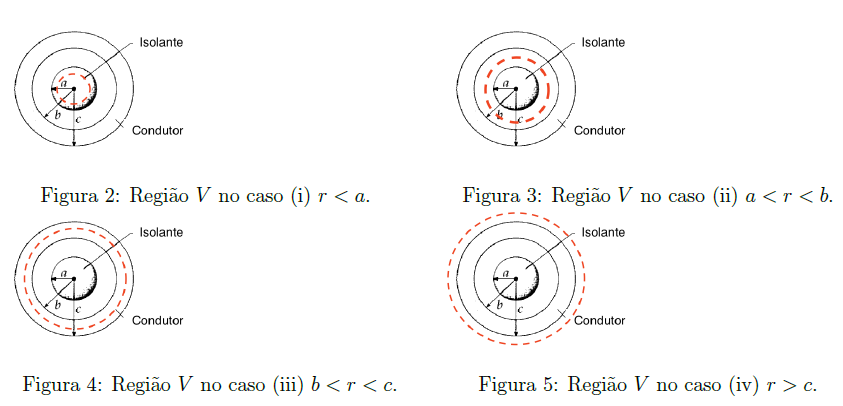
\includegraphics[scale=1]{eletromag-img/imagens.png}
  \caption{figuras}\label{figuraspng}
\end{figure}

b) Ache a carga induzida por unidade de área nas superfícies interna e externa do condutor.

\resposta Em todo condutor em equilíbrio eletrostático, a carga líquida se distribui na sua superfície. Vamos denotar por $q_{1}$ a carga induzida na superfície interna do condutor ($r = b$) e $q_{2}$ a carga induzida na superfície externa do condutor ($r = c$). Como dentro do condutor temos $E = 0$, aplicando a Eq. (\ref{eq9}) a uma região como as do item (a)(iii) (raio $r$, tal que $b < r < c$), a carga total em $V$ nesse caso é nula. Portanto,
%
\begin{equation}
  q_{V} = Q + q_{1} = 0 \ \ \ q_{1} = - Q .
\end{equation}
%
Como, por simetria, a carga se distribui de maneira uniforme na superfície, segue que a densidade de carga induzida em $r = b$ é
%
\begin{equation}
  \sigma_{1} = - \frac{Q}{ 4 \pi b^{2} } .
\end{equation}
%
Como o condutor está descarregado, por conservação de carga, temos que
%
\begin{equation}
  \begin{array}{ccc}
    Q_{condutor} & = & q_{1} + q_{2} \\
    q_{2} & = & - q_{1}
  \end{array}
\end{equation}
%
Usando novamente que, por simetria, a carga se distribui de maneira uniforme na superfície, a densidade de carga induzida em $r = c$ é
\begin{equation}
  \sigma_{2} = \frac{Q}{4 \pi c^{2}} .
\end{equation}



c) Esboce o gráfico da magnitude do campo elétrico $E$ versus $r$. Identifique em seu gráfico cada uma das regiões citadas no item (a).

\resposta Esboço do gráfico $E \times r$:
%
\begin{figure}[H]
  \centering
  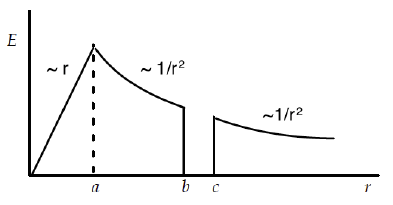
\includegraphics[scale=1]{eletromag-img/esboco.png}
  \caption{Esboço do gráfico $E \times r$.}\label{esbocopng}
\end{figure}
%





\item Considere as equações de Maxwell na forma diferencial e resolva cada item abaixo.


a) Derive, mostrando todos os passos, as equações de onda no vácuo em sua forma vetorial para os campos elétrico e magnético. Lembre-se:
$$
\boldsymbol{ \nabla \times (\nabla \times V) = \nabla ( \nabla \cdot V ) - \nabla^{2} V } \mbox{ e  } \boldsymbol{ \nabla \cdot (\nabla \times V) = 0}
$$

\resposta Pelo formulário podemos ver que no vácuo (onde $\rho = 0$ e $\vec{J} = 0$), as equações de Maxwell são dadas por
%
\begin{eqnarray}
% \nonumber % Remove numbering (before each equation)
  \nabla \cdot \vec{E} &=& 0; \label{eq10} \\
  \nabla \cdot \vec{B} &=& 0; \label{eq11} \\
  \nabla \times \vec{E} &=& - \frac{\partial \vec{B}}{\partial t}; \label{eq12} \\
  \nabla \times \vec{B} &=& - \mu_{o} \epsilon_{o} \frac{\partial \vec{E}}{\partial t} . \label{eq13}
\end{eqnarray}
%
Tomando o rotacional da Eq. (\ref{eq12}) temos que
%
\begin{equation}\label{eq14}
  \nabla \times (\nabla \times \vec{E}) + \nabla \times \left( \frac{\partial \vec{B}}{\partial t}  \right) = 0 .
\end{equation}
%
Utilizando a primeira identidade vetorial dada no enunciado juntamente com a Eq. (\ref{eq10}), podemos re-escrever o primeiro termo do lado esquerdo da equação acima como
%
\begin{equation}
  \nabla \times (\nabla \times \vec{E}) = \nabla (\nabla \cdot \vec{E}) - \nabla^{2} \vec{E} = - \nabla^{2} \vec{E} .
\end{equation}
%
Desta forma a Eq. (\ref{eq14}) pode ser re-escrita, trocando a ordem das derivadas parciais, como
%
\begin{equation}
  -  \nabla^{2} \vec{E} + \frac{\partial}{\partial t} (\nabla \times \vec{B}) = 0 .
\end{equation}
%
Utilizando a Eq. (\ref{eq13}) obtemos a equação da onda para o campo elétrico
%
\begin{equation}
  \nabla^{2} \vec{E} = \mu_{o} \epsilon_{o} \frac{\partial^{2} \vec{E}}{\partial t^{2}} .
\end{equation}
%
Tomando agora o rotacional da Eq. (\ref{eq13}) temos que
%
\begin{equation}
  \nabla \times (\times \times \vec{B}) - \mu_{o} \epsilon_{o} \nabla \times \left( \frac{\partial \vec{E} }{\partial t}  \right) = 0 .
\end{equation}
%
Utilizando a primeira identidade vetorial dada no enunciado juntamente com a Eq. (\ref{eq11}) e trocando a ordem das derivadas parciais, podemos re-escrever a equação acima como
%
\begin{equation}\label{eq15}
  - \nabla^{2} \vec{B} - \mu_{o} \epsilon_{o} \frac{\partial}{\partial t} (\nabla \times \vec{E}) = 0 .
\end{equation}
%
Finalmente, utilizando a Eq. (\ref{eq12}) no segundo termo da Eq. (\ref{eq15}) obtemos
%
\begin{equation}
  \nabla^{2} \vec{B} = \mu_{o} \epsilon_{o} \frac{\partial^{2} \vec{B}}{\partial t^{2}} .
\end{equation}
%


b) Escreva a equação de onda para uma função escalar qualquer $f(\vec{r},t)$ e, comparando com as expressões obtidas no item (a), determine a velocidade de propagação para ambos os campos.

\resposta A equação de onda para uma função $f(\vec{r},t)$ se propagando com velocidade $v$ é dada por
%
\begin{equation}\label{eq16}
  \nabla^{2} f (\vec{r},t) = \frac{1}{v^{2}} \frac{\partial^{2} f (\vec{r},t) }{\partial t^{2}} .
\end{equation}
%
Comparando com as Eqs. (\ref{eq15}) e (\ref{eq16}), notamos que a velocidade de propagação de $\vec{E}$ e $\vec{B}$ é dada por
%
\begin{equation}\label{eq17}
  \frac{1}{v^{2}} = \mu_{o} \epsilon_{o} \Rightarrow \ \  v  = \frac{1}{\sqrt{\mu_{o} \epsilon_{o} }} = c.
\end{equation}
%



c) Uma possível solução da equação obtida no item (a) é a solução do tipo onda plana linearmente polarizada. Suponha um campo eletromagnético do tipo onda plana linearmente polarizada que esteja se propagando na direção $\hat{z}$. Considerando que $\omega$ é a frequência angular, $k$ o número de onda, $E_{0}$ e $B_{0}$ as amplitudes dos campos elétrico e magnético, respectivamente, escreva explicitamente qual é o módulo e a direção de $\vec{E}$ e $\vec{B}$ em função da posição e do tempo.

\resposta Supondo que $\vec{E}$ aponte na direção $\hat{x}$ e se propague na direção $\hat{z}$, podemos escrever que
%
\begin{equation}
\begin{array}{ccc}
  \vec{E} &=& E_{o} e^{i (kz - \omega t)} \hat{x} , \\
  \vec{B} &=& B_{o} e^{i(kz - \omega t)} \hat{y} \label{eq19} .  
\end{array}
\end{equation}
%
Os campos "físicos" podem ser escritos como (supondo $E_{o}$ e $B_{o}$ reais)
%
\begin{equation}
\begin{array}{ccc}
  \vec{E} &=& Re(\vec{E}) = E_{o} \cos (kz - \omega t) \hat{x} , \\
  \vec{B} &=& Re(\vec{B}) = B_{o} \cos (kz - \omega t) \hat{y} . \label{eq21} .
\end{array}
\end{equation}
%
Essas soluções, de fato, satisfazem as quatro Eqs. (10-13) desde que $ \omega = c k$, como pode ser verificado. De maneira geral, a direção de $\vec{E}$ é arbitrária, desde que seja perpendicular a $\vec{z}$. Uma vez fixada a direção de $\vec{E}$, $\vec{B}$ tem que ser perpendicular a $\vec{E}$ e $\vec{z}$. Os módulos de $\vec{E}$ e $\vec{B}$ são:
%
\begin{equation}
\begin{array}{ccc}
  E & = & E_{o} \cos(kz - \omega t), \\
  B & = & B_{o} \cos(kz - \omega t) .
\end{array}
\end{equation}
%

d) Partindo agora das equações de Maxwell na presença de cargas e correntes, derive a equação que relaciona as densidades de carga e de corrente elétrica (equação da continuidade). Que lei de conservação é expressa matematicamente por esta equação?


\resposta Tomando a divergência da Eq. (\ref{eq13}) temos
%
\begin{equation}\label{eq22}
  \nabla \cdot (\nabla \times \vec{B}) - \mu_{o} \epsilon_{o} \frac{\partial}{\partial t} (\nabla \cdot \vec{E}) = \mu_{o} \nabla \cdot \vec{J} .
\end{equation}
%
O primeiro termo se anula pela segunda identidade dada no enunciado. Usando a Eq. (\ref{eq10})
%
\begin{equation}
  \frac{\partial \rho}{\partial t} + \nabla \cdot \vec{J} = 0
\end{equation}

Esta equação expressa a lei de \textit{conservação da carga}: em sua forma integral, ela implica que a taxa de variação temporal da carga total incluída em uma região espacial fixa é igual ao fluxo de corrente elétrica entrando pela superfície que delimita a região.



\item {a)} Um cilíndrico dielétrico maciço, de comprimento infinito e raio $a$, possui uma densidade de carga volumétrica uniforme e positiva $\rho$. Uma casca cilíndrica, também dielétrica, de raio $b > a$, com eixo comum ao cilindro, tem uma densidade de carga superficial uniforme e negativa $\sigma$, de forma que a carga total do cilidro mais casca, em certo comprimento, é zero, e portanto $ \sigma = -\rho a^{2} / 2b$. Calcule o campo elétrico $\vec{E}(r)$ para as regiões $r < a$, $a < r < b$ e $b < r$ sendo $r$ a distância ao eixo do cilindro.


\resposta

b) Considere em seguida que o conjunto cilindro mais casca se move para a direita com velocidade $\vec{v}$. O movimento dá origem a uma corrente elétrica $I = \pi a^{2} \rho v$ no cilindro maciço, para a direita e uniformemente distribuida na seção reta, de forma que a densidade de corrente fica sendo dada por $\vec{J} = \rho \vec{v}$. Da mesma forma, a casca em movimento dá origem a uma corrente de mesma intensidade $I$, mas em sentido contrário (para a esquerda). Calcule a indução magnética $\vec{B}$ para as regiões $r < a$, $a < r < b$ e $b < r$.


\begin{figure}[H]
\centering
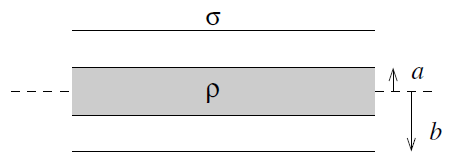
\includegraphics[scale=1]{eletromag-img/inducao.png}
\end{figure}



\item O campo elétrico de uma onda plana monocromática no vácuo é dado por

$$
\vec{E}(z,t) = ( E_{1} \hat{x} + E_{2} \hat{y} )e^{i(kz - \omega t)}.
$$
onde $\hat{x}$ e $\hat{y}$ são versores cartesianos nas direções $x$ e $y$, respectivamente, e $E_{1}$ e $E_{2}$ sáo constantes.


a) Encontre a indução magnética $\vec{B}(z,t)$.

\resposta

b) Mostre que o campo elétrico e a indução magnética são ortogonais entre si.

\resposta

c) Encontre o vetor de Poynting da onda.

\resposta


\item Uma espira condutora retangular (comprimento $a$, largura $b$ e resistência $R$) situa-se nas vizinhanças de um fio reto infinitamente longo que é percorrido por uma corrente $i$ para a direita, conforme a figura. A espira afasta-se do fio com uma velocidade constante $\vec{v}$, de forma que a distância do centro da espira ao fio é dada por $s(t) = s_{0} + vt$. Calcule:


a) o módulo do campo magnético produzido pela corrente num ponto situado a uma distância $r$ do fio. Indique a direção e o sentido do campo na região delimitada pela espira;

\resposta

b) o fluxo magnético na região delimitada pela espira para um dado valor de $s(t)$;

\resposta

c) a força eletromotriz induzida na espira para uma certa distância $s(t)$;

\resposta

d) a corrente induzida na espira, $i_{ind}$. Indique o sentido da mesma.

\begin{figure}[H]
\centering
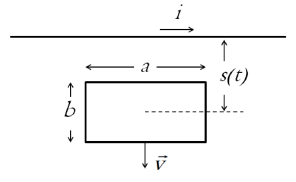
\includegraphics[scale=1]{eletromag-img/espira2.png}
\end{figure}


\resposta


\item Um meio condutor tem condutividade elétrica $\sigma$, permeabilidade magnética $\mu_{0}$ e permissividade elétrica $\epsilon = K \epsilon_{0}$, em que $K$ é a constante dielétrica real. A equação de onda para o campo elétrico neste meio é dada por $\nabla^{2} \vec{E} - K \frac{1}{c^{2}} \frac{\partial^{2} \vec{E}}{\partial t^{2}} -  \frac{\sigma}{\epsilon_{0}} \frac{1}{c^{2}} \frac{\partial \vec{E}}{\partial t} = 0$, sendo $\frac{1}{c^{2}} = \mu_{0} \epsilon_{0}$.


a) Mostre que a função de onda plana monocromática $\vec{E}(z,t) = \vec{E_{0}}e^{i(\omega t - \tilde{q} z)}$ é solução da equação diferencial acima. Encontre a relação entre o número de onda complexo, $\tilde{q}$, e a frequência angular, $\omega$, para que $\vec{E}(z,t)$ seja solução. Mostre também que $\tilde{q}$ se torna real no caso de um meio isolante.

\resposta

b) Encontre a constante dielétrica complexa, $\tilde{K}$, usando a relação entre o número de onda e a constante dielétrica, $\tilde{q}^{2} = \tilde{K} \frac{\omega^{2}}{c^{2}}$. Verifique que a parte real de $\tilde{K}$ é igual a $K$ , como esperado, e explicite a parte imaginária de $\tilde{K}$.

\resposta

c) Faça a aproximação para baixas frequências na expressão da constante dielétrica complexa do item (b) e calcule o índice de refração complexo, $\tilde{n} = \sqrt{\tilde{K}}$. Mostre que as partes real e imaginária de $\tilde{n}$ são iguais neste caso.

\resposta

d) A profundidade de penetração da onda no meio condutor, $\delta$, é dada pelo inverso da parte imaginária do número de onda, $q_{i}$, ou seja, $\delta = 1/q_{i}$. Lembre-se de que $\tilde{q} = \tilde{n} \frac{\omega}{c}$ e calcule a profundidade de penetração para a prata ($Ag$) na região de micro-ondas ($f = \frac{\omega}{2\pi} = 10 GHz$), para a qual vale a aproximação do item (c). A condutividade da prata nesta faixa de frequências é $ \sigma_{Ag} = 3 \times 10^{+7}(\Omega m)^{-1}$. Aproxime o resultado do cálculo e obtenha a ordem de grandeza de $\delta_{Ag} (1 m, 10 cm, 1 cm ...)$.



\item Considere um condutor macroscópico de forma arbitrária, cuja superfície é fechada e suave. Partindo da lei de Gauss e considerando que o rotacional do campo eletrostático é nulo:


a) Calcule o campo elétrico no interior do condutor;

\resposta

b) Obtenha a componente normal do campo elétrico na superfície externa do condutor em termos da densidade superficial de carga;

\resposta

c) Obtenha a componente tangencial do campo elétrico na superfície do condutor.

\resposta



\item Considere um conjunto de soluções de ondas planas eletromagnéticas no vácuo, cujos campos (elétrico e magnético) são descritos pela parte real de funções: $\vec{u}(\vec{x},t) = \vec{A}e^{i(\vec{k} \cdot \vec{x} - \omega t)}$, onde $\vec{k}$ é o vetor de onda, que determina a direção de propagação da onda, e $\omega$ é a frequência angular, que se relaciona com o vetor de onda por $\omega = v |\vec{k}|$, onde $v = 1 / \sqrt{\epsilon \mu}$ é a velocidade de propagação das ondas.


a) Mostre que o divergente de $\vec{u}(\vec{x},t)$ satisfaz: $\vec{\nabla} \cdot \vec{u} = i \vec{k} \cdot \vec{u}$;

\resposta

b) Mostre que o rotacional de $\vec{u}(\vec{x},t)$ satisfaz: $\vec{\nabla} \times \vec{u} = i \vec{k} \times \vec{u}$;

\resposta

c) Demonstre que as ondas são transversais e que os vetores $\vec{E}$ , $\vec{B}$ e $\vec{k}$ são mutuamente perpendiculares.

\resposta



\item Um capacitor esférico é composto por uma esfera condutora de raio $R_{1}$, concêntrica com uma casca condutora esférica de raio $R_{2}$ e espessura desprezível, com $R_{1} < R_{2}$. O condutor interno possui carga $+Q$ e o externo possui carga $-Q$.


a) Calcule o campo elétrico e a densidade de energia em função de $r$, onde $r$ é a distância radial a partir do centro dos condutores, para qualquer $r$.

\resposta

b) Determine a capacitância $C$ do capacitor.

\resposta

c) Calcule a energia do campo elétrico armazenada em uma casca esférica de raio $r$, espessura $dr$ e volume $4\pi r^{2}dr$, localizada entre os condutores. Integre a expressão obtida para encontrar a energia total armazenada entre os condutores. Dê sua resposta em termos da carga $Q$ e da capacitância $C$.

\resposta


\item Duas bobinas idênticas, compostas cada uma por um anel de raio $R$ e espessura desprezível, são montadas com seus eixos coincidentes com o eixo$-z$, conforme se vê na figura abaixo. Seus centros estão separados por uma distância $d$, com o ponto médio P coincidindo com a origem do eixo$-z$. Cada bobina transporta uma corrente elétrica total de intensidade I. Ambas as correntes têm o mesmo sentido anti-horário.


a) Utilize a lei de Biot-Savart para determinar o campo magnético de uma única bobina ao longo de seu eixo de simetria.

\resposta

b) A partir do resultado anterior, obtenha o campo magnético $B(z)$ ao longo do eixo$-z$ das duas bobinas.

\resposta

c) Admitindo que o espaçamento $d$ seja igual ao raio $R$ das bobinas, mostre que, no ponto $P$, as seguintes igualdades são válidas: $dB/dz = 0$ e $d^{2}B/dz^{2} = 0$.

\resposta

d) Considerando os gráficos abaixo, de $B$ (em unidades arbitrárias) versus $z$, qual curva descreve o campo magnético ao longo do eixo$-z$ na configuração do item (b)? Justifique.

\resposta

e) Supondo que a corrente na bobina superior tenha seu sentido invertido, calcule o novo valor do campo magnético no ponto P.

\begin{figure}[H]
\centering
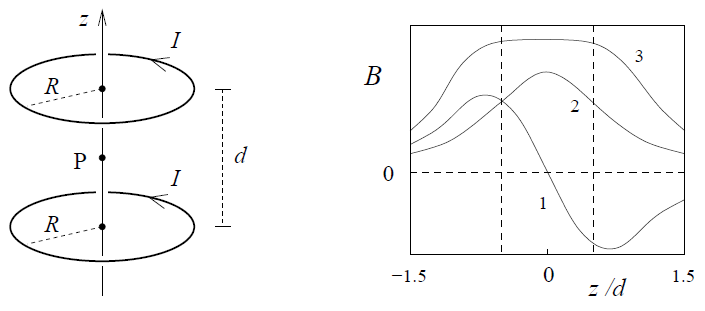
\includegraphics[scale=0.8]{eletromag-img/espira3.png}
\end{figure}

\resposta



\item Considere uma esfera sólida, uniformemente carregada, de carga $Q$ e raio $R$.


a) Determine o vetor campo elétrico $\vec{E}$ em um ponto à distância $r$ do centro da esfera, nos casos $r > R$ e $r \leq R$.

\resposta

b) Obtenha a força $d \vec{F}$ sobre um elemento de volume $dV$ da esfera, localizado na posição $\vec{r}$.

\resposta

c) Determine agora, por integração, a força total $\vec{F}$ que age sobre o hemisfério superior da esfera.

\resposta



\item Um capacitor de placas planas paralelas é formado por dois discos circulares de raio $a$, separados entre si de uma distância $d << a$, no vácuo. As placas estão ligadas a um gerador de corrente alternada de frequência $\omega$, que produz uma carga uniforme na placa do capacitor, dada por $q(t) = q_{0} sin(\omega t)$. São desprezados efeitos de borda. Supondo baixas frequências, de forma que $\omega a/c << 1$ (onde $c = 1/\sqrt{\mu_{0} \epsilon}$ é a velocidade da luz), o campo elétrico $\vec{E}$ entre as placas pode ser considerado uniforme. Considere um sistema de coordenadas cilíndricas, ($r,\theta,z$), com eixo $z$ passando pelo centro das placas, conforme indicado na figura.

\begin{figure}[H]
\centering
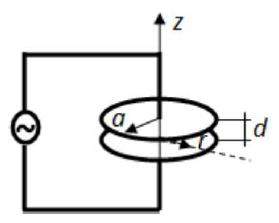
\includegraphics[scale=0.8]{eletromag-img/paralela.png}
\end{figure}


a) Calcule a expressão para o campo elétrico $\vec{E}$ entre as placas.

\resposta

b) Calcule o campo magnético $\vec{B}$, em função do raio $r$, na região entre as placas do capacitor.

\resposta

c) Calcule o vetor de Poynting $\vec{S} = (\vec{E} \times \vec{B} )/\mu_{0}$.

\resposta

d) Usando a aproximação de baixas frequências, mostre que é satisfeita a conservação de energia, expressa pela condição $\Delta \cdot \vec{S} + \partial u / \partial t = 0 $, onde $u = \frac{1}{2} ( \epsilon_{0} \vec{E}^{2} + \vec{B}^{2}/\mu_{0} )$ é a densidade de energia contida no campo eletromagnético.

\resposta


\item Considere um fio infinitamente longo disposto paralelamente ao eixo $z$, interceptando o plano $z = 0$ em $x = a$ e $y = 0$, conforme mostra a figura. O fio está carregado com densidade linear de carga elétrica $\lambda$ uniforme.

\begin{figure}[H]
\centering
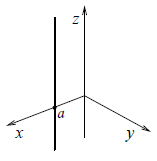
\includegraphics[scale=0.8]{eletromag-img/fio.png}
\end{figure}


a) Determine o potencial elétrico $V (x,y,z)$ em todo o espaço, de forma que o potencial seja zero no eixo $z$. Sugestão: pode-se calcular o potencial a partir do campo elétrico do fio longo, que é obtido de forma simples usando a lei de Gauss.

\resposta

b) Considere agora, além do fio, um condutor plano infinito (aterrado) ocupando o plano $x = 0$. Calcule $V (x,y,z)$ para a região $x > 0$ do espaço. Sugestão: utilize o método das imagens.

\resposta

c) Qual a densidade superficial de carga $\sigma(y,z)$ induzida no condutor plano em $x = 0$?

\resposta

d) Calcule a integral $\int_{-\infty}^{\infty} \sigma (y,z) dy$ e discuta o resultado obtido.

\resposta



\item Um fio carregado com densidade linear de carga elétrica $\lambda > 0$ está colado (formando um anel) na borda de um disco isolante de raio $a$, que pode girar ao redor de seu eixo vertical sem atrito. O comprimento do fio é exatamente $2\pi a$. Apenas na região central do disco, até um raio $b < a$, age um campo magnético uniforme $\mathbf{B_{0}}$ vertical para cima.

\begin{figure}[H]
\centering
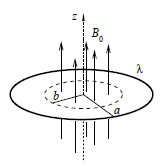
\includegraphics[scale=0.8]{eletromag-img/fio1.png}
\end{figure}


a) O campo magnético é agora desligado. Obtenha a expressão para o torque devido à força eletromotriz induzida no fio, em termos da variação temporal do campo magnético, $d\mathbf{B}/dt$. A partir deste resultado, calcule o momento angular final do disco (módulo e direção).

\resposta

b) Considerando como dado o momento de inércia $I$ do sistema disco$+$fio, calcule o campo magnético (módulo e direção) produzido no centro do disco pelo anel de carga na situação final acima.

\resposta


\item Um cabo coaxial é composto por um longo cilindro reto condutor de raio $a$ e uma fina casca cilíndrica condutora de raio $b$ e concêntrica ao cabo interno. Os dois condutores transportam correntes iguais e opostas de intensidade $i$.


a) Determine o módulo do campo magnético na região entre os dois condutores ($a < r < b$).

\resposta

b) Determine o módulo do campo magnético na região externa ao cabo coaxial ($r > b$).

\resposta

c) Encontre o módulo do campo magnético no interior do cilindro interno ($r < a$) se a corrente está distribuída uniformemente na seção transversal do mesmo.

\resposta

d) Calcule a energia armazenada no campo magnético por unidade de comprimento do cabo.

\resposta


\item Um capacitor esférico isolado possui carga $+Q$ sobre o condutor interno (raio ra) e carga $-Q$ sobre o condutor externo (raio $r_{b}$). A seguir, a metade inferior do volume entre os dois condutores é preenchida por um líquido de constante dielétrica relativa $K$, conforme indicado na seção reta da figura abaixo.

a) Calcule o módulo do campo elétrico no volume entre os dois condutores em função da distância $r$ ao centro do capacitor. Forneça respostas para a metade superior e para a metade inferior desse volume.

\resposta

b) Determine a densidade superficial de cargas livres sobre o condutor interno e sobre o condutor externo.

\resposta

c) Calcule a densidade superficial de cargas de polarização sobre as superfícies interna ($r_{a}$) e externa ($r_{b}$) do dielétrico.

\resposta

d) Qual é a densidade de carga de polarização sobre a superfície plana do dielétrico? Explique.

\resposta

e) Determine a capacitância do sistema.
\begin{figure}[H]
\centering
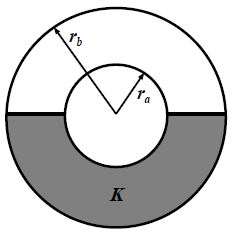
\includegraphics[scale=0.8]{eletromag-img/espira4.png}
\end{figure}

\resposta


\item Um cilindro de altura $h$ e raio externo $b$ é feito de um material com condutividade elétrica $\sigma$ e permissividade elétrica $\epsilon$. O cilindro é furado ao longo de seu eixo de forma que seu raio interno é $a$. Um material de alta condutividade elétrica preenche o furo central do cilindro e
forma também uma casca cilíndrica em torno da sua borda externa, formando os contatos elétricos do cilindro, conforme ilustra a figura abaixo. Considere $h >> b$, de modo que os efeitos de borda podem ser desprezados. Aplica-se uma diferença de potencial elétrico $V_{0}$ entre esses contatos (tome $V = 0$ na superfície externa do cilindro).



a) Mostre que, no regime estacionário ($\frac{\partial \rho}{\partial t} = 0$), a densidade de carga no interior do meio condutor homogêneo é nula.

\resposta

b) Mostre que, nesse caso, o potencial elétrico obedece à equação de Laplace e obtenha o vetor campo elétrico $\vec{E}(\vec{r})$ no interior do cilindro.

\resposta

c) Calcule a carga livre total acumulada na superfície do contato interno (raio $a$) e a capacitância entre os dois contatos elétricos.

\resposta

d) Calcule a resistência elétrica entre esses dois contatos elétricos.
\begin{figure}[H]
\centering
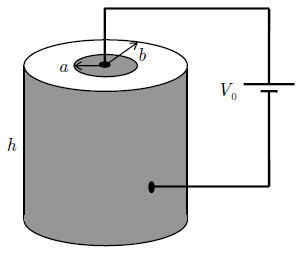
\includegraphics[scale=0.6]{eletromag-img/capacitor.png}
\end{figure}

\resposta



\item Um cilindro condutor muito longo de raio $a$ conduz uma corrente $I$ ao longo de seu eixo $z$. A densidade de corrente $\vec{J}$ no interior do cilindro varia de acordo com a expressão abaixo:
$$
\vec{J}(r, \varphi, z)=\hat{z} \frac{J_{0}}{r} \operatorname{sen}\left(\frac{\pi r}{a}\right)
$$
onde $r$ é a distância radial entre o ponto considerado e o eixo do cilindro.

a) Determine a constante $J_{0}$ em termos de $I$ e $a$.

\resposta

b) Calcule o campo magnético $\vec{B}$ fora do cilindro condutor ($r > a$) e expresse seu resultado em termos de $I$ e $a$.

\resposta


c) Calcule o campo magnético $\vec{B}$ no interior do cilindro condutor ($r < a$) e expresse seu resultado em termos de $I$ e $a$.

\resposta

d) Esboce um gráfico qualitativo do módulo do campo magnético, $B(r)$, indicando seu comportamento em $r = 0$ e $r = a$.

\resposta



\item Coloca-se uma esfera metálica descarregada, de raio $R$, numa região do espaço inicialmente preenchida por um campo elétrico dado por $\vec{E}_{i} = E_{0} \ \hat{k}$. Escolha a origem do sistema de coordenadas no centro da esfera.

a) Esboce as linhas do campo elétrico em toda a regi˜ao do espaço. Justifique o esboço utilizando argumentos físicos.

\resposta

b) Determine o campo elétrico $\vec{E}_{f} (\vec{r})$ em toda a região do espaço. Em particular, encontre os campos para os pontos em que $|\vec{r}| >> R$ e $|\vec{r}| >> R$ e verifique se eles s˜ao consistentes com o esboço no item (a).

\resposta

c) Ache a densidade de carga na esfera. Se a esfera possuir raio igual a $10 \ cm$ e $E_{0} = 100 \ N/C$, calcule as cargas acumuladas nos hemisférios norte e sul da esfera.

\resposta

d) Suponha que a esfera metálica seja substituída por uma esfera dielétrica. Discuta qualitativamente o que ocorre neste caso e esboce as linhas do campo elétrico em toda a região do espaço.

\resposta

\item Considere o arranjo hipotético ilustrado na figura abaixo, em que um fio sólido de raio $a$ estendido ao longo do eixo $z$ conduz uma corrente elétrica $I$, uniformemente distribuída sobre a sua seção transversal, que é mantida constante. A pequena lacuna no fio, de largura $w << a$, forma um capacitor de placas paralelas. A carga no capacitor é zero no instante $t = 0$.

a) Encontre o vetor campo elétrico na lacuna em função da distância $\rho$ a partir do eixo $z$ e do tempo $t$, além dos parâmetros $I$, $w$ e $a$. Despreze os efeitos de borda.

\resposta

b) Encontre o vetor campo magnético na lacuna em função de $\rho$ e $t$ e dos parâmetros $I$, $w$ e $a$.

\resposta

c) Calcule a densidade de energia eletromagnética $u_{em}$ e o vetor de Poynting na lacuna, indicando explicitamente a sua direção e o seu sentido.

\resposta

d) Determine a energia total $U_{em}$ na lacuna em função do tempo. Compare a taxa de variação de $U_{em}$ com o tempo e o fluxo de energia por unidade de tempo (fluxo de potência), obtido fazendo-se a integral de superfície do vetor de Poynting.

\begin{figure}[H]
\centering
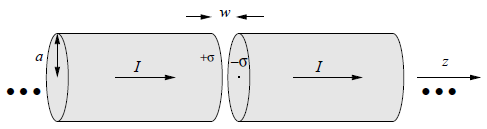
\includegraphics[scale=0.8]{eletromag-img/solido.png}
\end{figure}

\resposta



\item Em uma fábrica de chocolate em pó, utiliza-se tubulações com ar comprimido para mover o chocolate em pó entre diferentes setores. Entretanto, com o atrito, o chocolate acaba ficando eletricamente carregado, de tal forma que temos uma densidade volumétrica uniforme de cargas positivas $\rho$ dentro da tubulação de raio $R$. Suponha que os tubos são condutores e encontram-se aterrados, e que a constante dielétrica do ar não é alterada pelo chocolate em pó.

a) Calcule o campo elétrico dentro e fora da tubulação, considerando que esta é um cilindro muito longo.

\resposta

b) Calcule o potencial elétrico dentro e fora da tubulação. Tome $V = 0$ na parede do tubo.

\resposta

c) Esboce o gráfico do campo elétrico e do potencial em função da distância ao eixo da tubulação.

\resposta

d) Se o campo elétrico for maior que um certo valor $E_{0}$, podemos ter o rompimento da rigidez dielétrica do ar, resultando numa faísca elétrica. Como o chocolate em pó é muito inflamável, uma faísca no interior da tubulação poderia causar uma explosão. Determine qual condição deve satisfazer para evitar este risco.

\resposta


\item Um plasma pode ser pensado como um gás clássico (não relativístico) de íons positivos e elétrons. Estamos interessados inicialmente na interação de uma onda eletromagnética com os elétrons livres deste plasma, já que estes têm massa muito menor do que os íons positivos.

a) Para uma onda eletromagnética harmônica transversal, seu campo elétrico $\vec{E}$ pode ser expresso na forma:
$$
\vec{E} = \vec{E}_{0} e^{i(\vec{k} \cdot \vec{r} - \omega t)}.
$$
Mostre que nas operações envolvendo $\vec{\nabla}$ este operador pode ser substituído por $i\vec{k}$, e as derivadas temporais $\frac{\partial}{\partial t}$ por $-i \omega$. Reescreva as equações de Maxell usando estes fatos.

\resposta

Considere que a onda harmônica se propaga na direção $z$ e suponha que o número médio de elétrons por unidade de volume do plasma é $n$.

b) Mostre que a densidade de corrente induzida pelo campo elétrico da onda é
$$
\vec{J} = i \frac{ne^{2}}{m \omega} \vec{E},
$$
onde $e$ e $m$ são, respectivamente, a carga e a massa do elétron, e $\omega$ é a frequência da onda. Justifique cuidadosamente suas hipóteses.

\resposta

c) Partindo das equações de Maxwell, obtenha a relação de dispersão $\omega(k)$ para a propagação da onda.

\resposta

d) O plasma admite a propagação de ondas com quaisquer frequências? Justifique sua resposta.

\resposta



\item Considere um fio infinitamente longo, carregado uniformemente com carga negativa de densidade $\lambda$, ao longo do eixo $x$. Suponha que acima deste fio, na posição $\vec{r} = y_{1} \hat{j}$, exista uma carga puntiforme $q$ positiva. O fio e a carga estão em repouso no referencial $S$. Um segundo referencial, $S'$, está se movendo para à direita, com uma velocidade relativística de módulo $v$, como mostra a figura abaixo. Tome a velocidade da luz como sendo $c$.
\begin{figure}[H]
\centering
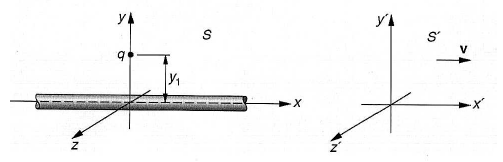
\includegraphics[scale=0.8]{eletromag-img/fio2.png}
\end{figure}

a) Calcule a força resultante, $\vec{F}_{res}$, atuando na carga $q$ no referencial $S$.

\resposta

b) Encontre a densidade de carga $\lambda '$ no referencial $S'$. Note que nesse referencial, o fio carregado está em movimento, o que implica na existência de uma corrente elétrica. Calcule essa corrente, indicando o sentido dela.

\resposta

c) Qual a força resultante, $\vec{F}'_{res}$, no referencial $S'$? Compare com $\vec{F}_{res}$, obtida no item (a). Quais as direções e sentidos dessas duas forças?

\resposta

d) A relação entre as forças eletromagnéticas $\vec{F}_{res}$ e $\vec{F}'_{res}$, obtidas nos itens (a) e (c), são consistentes com os resultados da teoria da relatividade? Justifique a sua resposta. \textit{Dica}: Pela teoria da relatividade restrita, as transformações entre $\vec{F}_{\perp}$ e $\vec{F}'_{\perp}$ e entre $\vec{F}_{\parallel}$ e $\vec{F}'_{\parallel}$, onde $\perp$ e $\parallel$ indicam as direções perpendiculares e paralela ao eixo $x$ (direção do movimento de $S'$), respectivamente, podem ser obtidas sabendo-se que (i) a energia e momento ($E,\vec{p}$) nos referenciais $S$ e $S'$ se transformam como o tempo e espaço ($t,\vec{r}$) e que (ii) a segunda lei de Newton, $\vec{F} = d\vec{p}/dt$ é válida também na relatividade restrita. Faça a transformação somente na direção de $\vec{F}_{res}$ e $\vec{F}'_{res}$.




\item Um condutor esférico maciço, de raio $a$ e carregado com carga $Q > 0$, está envolto por um material dielétrico esférico, de constante dielétrica $\epsilon_{r} = \epsilon / \epsilon_{0}$ e raio externo $b$, conforme mostra a figura abaixo.
\begin{figure}[H]
\centering
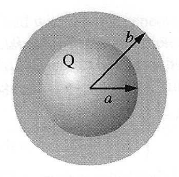
\includegraphics[scale=0.8]{eletromag-img/esfera2.png}
\end{figure}
a) Determine o campo elétrico em todo o espaço e esboce um gráfico de seu módulo $E(r)$.

\resposta

b) Determine o potencial no centro das esferas, tomando-se como zero o potencial no infinito.

\resposta

c) Encontre as distribuições das cargas livre e ligada (de polarização) nas esferas condutora e dielétrica. Faça uma figura mostrando onde as densidades de cargas se localizam, indicando se são positivas ou negativas.

\resposta

d) Calcule a energia eletrostática do sistema.

\resposta


\item Um cabo coaxial é constituído por um fio sólido de raio $a$ envolto por uma casca cilíndrica concêntrica de raio $b$, com comprimento $L >> b$. Ele é usado como linha de transmissão entre uma bateria de $fem$ $V$ e uma resistência $R$, como indicado na figura abaixo. Despreze a resistência do cabo.

a) Calcule o vetor campo elétrico no interior do cabo coaxial ($a < r < b$).

\resposta

b) Calcule o vetor campo magnético no interior do cabo coaxial ($a < r < b$).

\resposta

c) Calcule o vetor de Poynting, indicando esquematicamente os vetores $\vec{E}$ , $\vec{B}$ e $\vec{S}$ com relação à seção transversal do cabo coaxial. O que aconteceria se os pólos da bateria fossem invertidos?

\resposta

d) Usando o vetor de Poynting, calcule a potência que flui da bateria para o resistor e explique por que este resultado é esperado. Observação: Indique claramente as superfícies gaussianas e/ou caminhos de integração utilizados nos cálculos acima.

\begin{figure}[H]
\centering
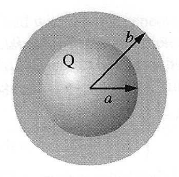
\includegraphics[scale=0.8]{eletromag-img/esfera2.png}
\end{figure}


\item Considere uma carga puntiforme $Q > 0$ a uma distância $D$ de uma placa infinita, condutora e aterrada, como ilustrada abaixo.

a) Desenhe as linhas de campo elétrico e as equipotenciais. Justifique seu desenho.

\resposta

b) Calcule as componentes $\hat{x}$ e $\hat{y}$ do vetor campo elétrico, em todo o espaço à esquerda da placa, em termos das componentes do ponto \textit{P} ilustrado na figura abaixo.

\resposta

c) Qual a densidade de carga na placa?

\resposta

d) Determine a força exercida pela placa sobre a carga \textit{Q}.

\begin{figure}[H]
\centering
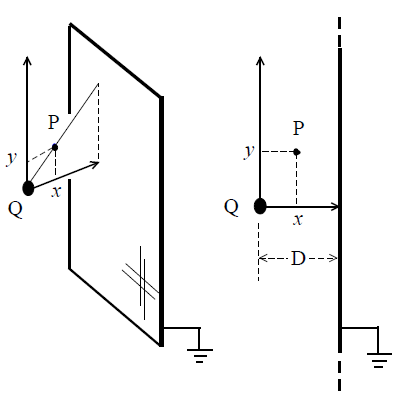
\includegraphics[scale=0.8]{eletromag-img/placa.png}
\end{figure}

\resposta


\item Dois planos semi-infinitos, isolados entre si, estão posicionados angularmente em $\phi = 0$ e $\phi = \pi/6$, sendo que $V(\phi = 0) = 0$ e $V(\phi = \pi/6) = 100 V$.

a) Utilizando a equação de Laplace mostre que, região entre as duas placas (para $r>0$), o potencial eletrostático é dado por: $V = (600/\pi)\phi$.

\resposta

b) obtenha a expressão do vetor campo elétrico correspondente.

\resposta

c) Calcule a força sofrida por um elétron, quando colocado ($v_{0} = 0$) entre as duas placas. Descreva a trajetória do elétron; esta trajetória corresponde a um arco de circunferência? Justifique!

\begin{figure}[H]
\centering
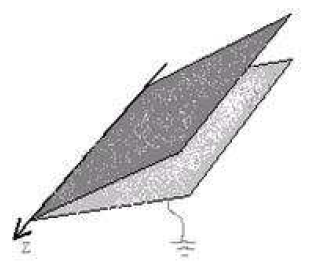
\includegraphics[scale=0.8]{eletromag-img/placas.png}
\end{figure}

\resposta

\item Uma haste de cobre de massa $m$ é posicionada sobre trilhos condutores terminados por um segmento condutor com resistência $R$, conforme a figura. Paralelamente aos trilhos, existe um fio muito longo que é percorrido por uma corrente $I_{1}$. Suponha que em $t=0$ a haste é impulsionada com uma velocidade $v_{0}$ e deixada livre para mover-se, sem atrito.
\begin{figure}[H]
\centering
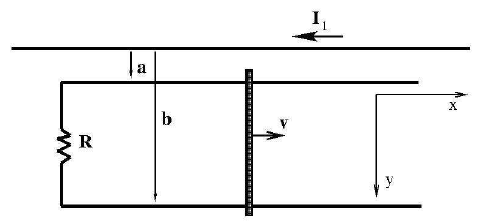
\includegraphics[scale=0.8]{eletromag-img/haste.png}
\end{figure}

a) Obtenha a expressão do campo magnético que atravessa a região da espira formada pela haste e os trilhos.

\resposta

b) Determine o sentido (horário/anti-horário) e o valor da corrente induzida na espira.

\resposta

c) Obtenha a expressão da velocidade da haste em função do tempo, em termos de $v_{0}$ e da constante $\tau$:
$$
\tau = \frac{4 \pi^{2} m R}{\mu_{0}^{2} I_{1}^{2} \operatorname{ln}^{2}(b/a)}
$$

\resposta


\item i) A partir das equações de Maxwell no vácuo:

a) Obtenha a equação de onda para o campo elétrico:
$$
\vec{\nabla}^{2} \vec{E} - \mu_{0} \epsilon_{0} \frac{\partial^{2} \vec{E}}{\partial t^{2}} = 0
$$

ii) Supor duas ondas eletromagnéticas planas, distintas, propagando-se na direção e sentido de $\hat{u}$ em um meio dielétrico com índice de refração $n=2$, com mesmas frequências e mesmos números de onda, que possuem respectivos campos elétricos dados por: $\vec{E}_{1} = E_{01} e^{-i(\omega t - K u)} \hat{p}$ e $\vec{E}_{2} = E_{02} e^{-i(\omega t - K u - \phi)} \hat{s}$.
\begin{figure}[H]
\centering
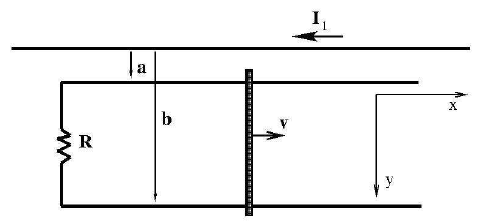
\includegraphics[scale=0.8]{eletromag-img/haste.png}
\end{figure}

\resposta

b) Discuta o estado de polarização de cada um destas ondas, em função dos possíveis valores da constante de fase $\phi$.

\resposta

c) Calcule o campo $\vec{B}$ e a média temporal do vetor de Poynting da onda resultante, correspondentes à superposição destas duas ondas.

\resposta


\item \textit{Experiência de Laboratório:} Um estudante decide medir a capacitância de um capacitor através de uma experiência calorimétrica. Ele aplica tensões variadas no capacitor, descarregando-o, logo em seguida, em um resistor $(R = 150 \Omega)$ mergulhado em um recipiente preenchido com óleo. Em cada etapa, o aumento de temperatura ocorrido no cunjunto óleo + resistor, após a descarga do capacitor, era cuidadosamente medida. Durante a execução de toda a experiência, o estudante também teve o cuidado de manter o conjunto (óleo e resistor, de Capacidade Térmica total $C_{T} = mc_{esp} = 200 J/ºC$) termicamente isolado do meio ambiente. A tabela de dados experimentais que ele obteve é mostrada abaixo.

\begin{center}
\begin{tabular}{|c|c|c|}
\hline
% after \\: \hline or \cline{col1-col2} \cline{col3-col4} ...
$\mathbf{V}[V]$ & $ \boldsymbol{\Delta T}[ºC] $ & $\boldsymbol{\sigma}_{\Delta T}[ºC]$ \\
50 & 0,1 & 0,1 \\ \hline
100 & 0,2 & 0,1 \\ \hline
150 & 0,3 & 0,1 \\ \hline
200 & 0,5 & 0,1 \\ \hline
250 & 0,6 & 0,1 \\ \hline
300 & 0,8 & 0,1 \\ \hline
350 & 1,1 & 0,1 \\ \hline
400 & 1,4 & 0,1 \\ \hline
450 & 1,7 & 0,1 \\ \hline
500 & 2,0 & 0,1 \\ \hline
\end{tabular}
\end{center}

a) Partindo do princípio de conservação de energia, mostre que a variação na temperatura do óleo é proporcional ao quadrado da tensão de carga dos capacitores: $\Delta T = \sigma V^{2}$; sendo $\alpha$ uma constante.

\resposta

b) Construa, no espaço quadriculado correspondente, um gráfico conveniente que lhe permite, a partir deste, obter o valor experimental da capacitância do capacitor utilizado pelo estudante na experiência.

\resposta

c) Como a experiência seria afetada caso o estudante resolvesse repetí-la utilizando um resistor do mesmo tipo só que com resistência $R' = 500 \Omega$? com qual destes resistores é possível realizar a experiência mais rapidamente?

\resposta


\item O betatron é um acelerador de elétrons, que se utiliza da força eletromotriz induzida por um campo magnético variável no tempo para acelerar os elétrons do feixe. Um campo magnético, também variável, serve para manter os elétrons em órbita circular. A figura 1 mostra um esquema do arranjo, visto de topo. Determine:
\begin{figure}[H]
\centering
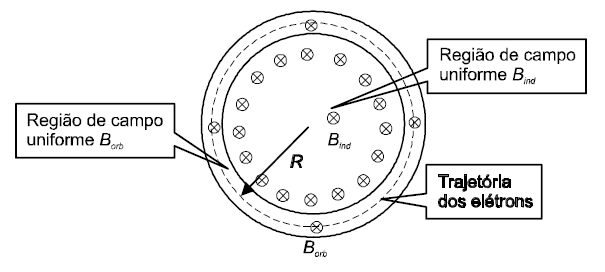
\includegraphics[scale=0.8]{eletromag-img/eletromotriz.png}
\caption{Esquema de um betatron em vista de topo}
\end{figure}

a) A relação entre $B_{ind}$ e $B_{orb}$ para que os elétrons, ao serem acelerados, permaneçam na órbita desejada que a região de campo $B_{ind}$ vale para $r<R$;

\resposta

b) A energia máxima do feixe, em $MeV$, para o caso de uma órbita com $R = 0,1 m$ e $B_{orb} = 0,5 T$ (considere o elétron ultra-relativístico);

\resposta

c) O valor do campo elétrico a que os elétrons estão submetidos durante o processo de aceleração, supondo que o processo de subida do campo magnético demore 1 $ms$.

\resposta


\item Um laser de alta potência, como o que está sendo projetado no IPEN, é capaz de produzir um pulso de $0,1 J$, com duração de $0,1 ps$. Considere que a luz tenha comprimento de onda de $1 \mu m$, seja linearmente polarizada na direção $x$, que o feixe se propague na direção $z$ e que tenha seção reta circular com raio $R = 0,5 \ cm$.

a) Determine, para um pulso, a densidade média de energia e o fluxo médio d energia.

\resposta

b) Calcule a amplitude dos campos elétrico e magnético da onda eletromagnética.

\resposta

c) Calcule a pressão exercida por um pulso que incide sobre uma superfície perfeitamente refletora.

\resposta

d) Escreva as expressões correspondentes para os vetores $\vec{E}(z,t)$ e $\vec{B}(z,t)$.

\resposta



\item Explique, de maneira simples, o que é usualmente conhecido como \textit{poder das pontas}, ou seja, que, próximo a uma superfície condutora, o campo elétrico será tão mais intenso quanto menor for o raio de curvatura da superfície (Justifique sua resposta).


\item Quando perguntado pela irmã mais nova sobre o funcionamento de uma tela de computador, um estudante de física esboçou o esquema de um tubo de raios catódicos, como mostrado na figura 1.

\begin{figure}[H]
\centering
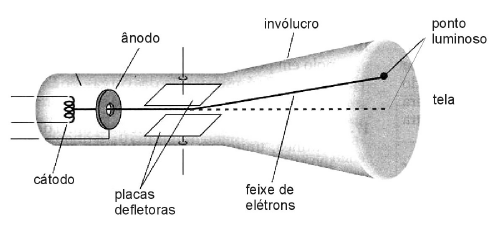
\includegraphics[scale=0.8]{eletromag-img/catodico.png}
\caption{Esquema de um tubo de raios catódicos}
\end{figure}

Explicou então a ela que os elétrons liberados pelo cátodo, a um potencial de $- kV$, são acelerados em direção ao ânodo, que, assim como o invólucro e a tela, está aterrado. Nessa situação os elétrons do feixe têm uma energia cinética de 1 $keV$. Ele também explicou o funcionamento das placas defletoras, que geram um campo elétrico vertical, o qual acelera os elétrons nessa direção, desviando-os da trajetória central. (Suponha que, para defletir o feixe para a extremidade da tela, as placas de deflexão tenham que ter uma $ddp$ de 10 $V$.) Afirmou, então, que os elétrons que chegam a uma das extremidades da tela têm uma energia cinética ligeiramente maior do que aqueles que chegam ao centro, por conta da aceleração experimentada entre as placas.

a) Que conceito(s) o estudante usou para fazer essa afirmação?

\resposta

b) Ele está correto? (Justifique suas resposta)

\resposta


\item Uma espira toroidal é mostrada na figura 2. Considere o enrolamento bem apertado, ou seja, que o campo magnético seja diferente de zero apenas no interior do toróide. Quando o meio em torno do qual a espira está enrolada é ferromagnético, a curva de $B \times H$ é mostrada na figura 3, iniciando com o material não magnetizado.

\begin{figure}[H]
\centering
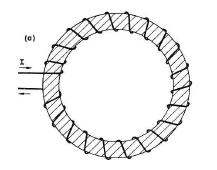
\includegraphics[scale=0.8]{eletromag-img/toroide.png}
\caption{Curvas $B \times H$.}
\end{figure}
\begin{figure}[H]
\centering
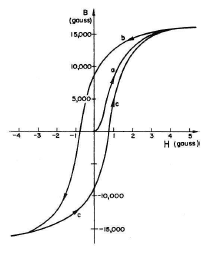
\includegraphics[scale=0.8]{eletromag-img/toroide2.png}
\caption{Curvas $B \times H$.}
\end{figure}

a) Explique fisicamente as curvas indicadas por $a$, $b$ e $c$.

\resposta

b) Esboce a curva que seria observada (e explique) caso a bobina fosse enrolada em torno de um meio não magnético e não condutor.

\resposta


\item Um capacitor de placas planas, paralelas e circulares, com raios $a$ e separação $d$ ($d << a$), tem capacitância $C = \frac{\epsilon_{0} \pi a^{2}}{d}$. Ele é ligado a uma bateria que fornece tensão $V_{0}$, através de fios retilíneos muito longos, de resistência total $R$, que coincidem com o eixo $z$, como mostrado na figura abaixo. Supondo que a bateria seja ligado em $t=0 \ s$:

a) Monte a equação diferencial relacionando a carga do capacitor com os elementos do circuito e mostre que a corrente no circuito é dada por $I(t) = \frac{V_{0}}{R} \operatorname{exp} \left( - \frac{t}{RC}  \right)$.

\resposta

b) Determine o vetor $\vec{E}(\rho, \phi, z, t)$ no interior do capacitor (supondo-o em vácuo e desprezando efeitos de borda).

\resposta

c) Usando a lei de Ampère e considerando a corrente de deslocamento, determine o vetor $\vec{B}(\rho, \phi, z, t)$ no interior do capacitor.
\begin{figure}[H]
\centering
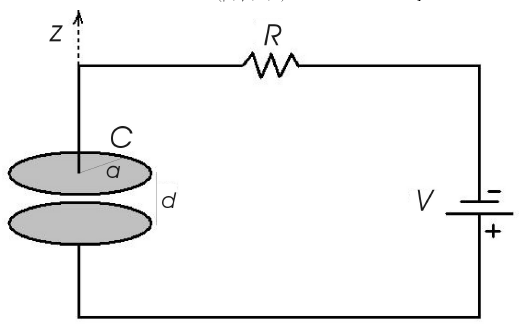
\includegraphics[scale=0.8]{eletromag-img/placaplana.png}
\caption{Circuito $RC$.}
\end{figure}

\resposta


\item O campo magnético de uma onda eletromagnética plana, no vácuo, é dado, em unidades do SI, por:
$$
\vec{B}(\vec{r}, t) = 10^{-6} (\hat{x} 2 \hat{y} + B_{z} \hat{z}) \operatorname{cos} (3x - y - z - \omega t)
$$
Determine:

a) A direção de propagação e o comprimento de onda.

\resposta

b) O valor da constante $B_{z}$.

\resposta


\item Um anel condutor de raio $R$ é colocado sobre o plano $xy$, centrado na origem. O campo magnético produzido por esse anel, ao longo do eixo $z$, quando por ele passa uma corrente $I$ no sentido $\phi$, é dado por:
$$
\vec{B}(z) = \frac{\mu_{0} I}{2} \frac{R^{2}}{ \left( R^{2} + Z^{2} \right)^{3/2}}
$$
A partir deste deste resultado, resolva o problema abaixo.

Considere agora um outro anel, de raio $a$, feito de material dielétrico e carregado uniformemente com carga $Q$. Esse anel está centrado na origem e tem um diâmetro ao longo do eixo $z$, em torno do qual é posto a girar com velocidade angular $\omega$ no sentido anti-horário ($\phi$), como mostrado na figura abaixo. Determine o vetor campo magnético na origem.

\begin{figure}[H]
\centering
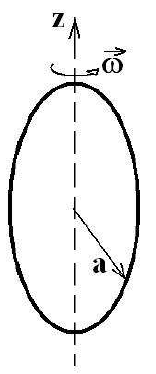
\includegraphics[scale=0.8]{eletromag-img/anel2.png}
\caption{Espira que gira em torno de $z$.}
\end{figure}



\item Explique o efeito de atração de um ímã por um material não magnético e condutor demonstrado na sala. Sua explicação deve conter: $a)$ indicação do fenômeno eletromagnético responsável pelo efeito; e $b)$ influência do movimento do ímã.



\item Considere um anel isolante de raio $a$ com massa $M$ e carga total $Q$ uniformemente distribuídas. O anel repousa sobre um plano horizontal sobre o qual pode se mover livremente sem atrito. Na região do anel há um campo magnético devido a uma fonte externa dado por:

$$
\vec{B}(t) = \left\{
\begin{array}{cc}
B_{0} \hat{e}_{z}, & \mbox{ se } t < 0, \\
B_{0} \hat{e}_{z} e^{-\alpha t}, & \mbox{ se } t \geq 0,
\end{array}
\right.
$$

onde $B_{0}$ e $\alpha$ são constantes positivas. O plano em que repousa o anel é o plano $xy$ e o centro do anel coincide com a origem do sistema de coordenadas. No instante $t=0$ o anel encontra-se parado.

a) Determine o campo elétrico sobre o anel como função do tempo.

\resposta

b) Encontre a velocidade angular do anel num instante $t > 0$. Desconsidere o campo produzido pelo anel em movimento.

\resposta

c) Há conservação de momento angular neste processo? Explique.

\resposta


\item Uma placa condutora aterrada se encontra no plano $xy$ ($z=0$). Uma carga $q$ é trazida até o ponto $d\hat{e}_{z}$, com $d > 0$. Determine:

a) o potencial eletrostático em todo o espaço;

\resposta

b) o campo elétrico em todo o espaço;

\resposta

c) a densidade de carga e a carga total induzida na superfície do condutor;

\resposta

d) o trabalho realizado para trazer a carga $q$ do infinito até o ponto $d\hat{e}_{z}$.

\resposta



\item As propriedades eletromagnéticas da ionosfera terrestre podem ser descritas por uma permeabilidade magnética $\mu = \mu_{0}$ e uma constante dielétrica $\epsilon_{0}$ dependente da frequência (angular) $\omega$ na forma
$$
\epsilon(w) = \epsilon_{0} \left(  1 - \frac{\omega_{0}^{2}}{\omega^{2}}   \right)
$$
O parâmetro $\omega_{0}$ é determinado pela composição da ionosfera. Considere uma onda plana numa determinada região da ionosfera cujo campo elétrico é dado por
$$
\vec{E} = E_{0} e^{i(kz - \omega t)}.
$$

a) Obtenha a relação de dispersão $k(\omega)$.

\resposta

b) Para que valores de $\omega$ uma onda eletromagnética propaga neste meio?

\resposta

c) Qual a velocidade de fase $v_{f}$ de uma onda eletromagnética neste meio?

\resposta

d) É possível que $v_{f}$ seja maior que a velocidade da luz no vácuo $c$? Explique.

\resposta

e) Qual a velocidade de grupo $v_{g}$ desta onda? Esta velocidade pode ser maior que $c$?

\resposta


\item Considere um cabo coaxial formado por duas cascas cilíndricas condutoras de raios $a$ e $b$ ($b > a$). Um material de permeabilidade magnética $\mu$ ocupa o espaço entre as cascas cilíndricas, que são percorridas por uma corrente constante $I$ ao longo de seu comprimento como mostra a figura abaixo. Determine:

a) O campo $\vec{H}$ em todo espaço;

\resposta

b) o campo magnético $\vec{B}$ em todo espaço;

\resposta

c) a magnetização $M$ em todo espaço;

\resposta

d) as correntes de magnetização em todo o espaço;

\resposta

e) a energia armazenada no cabo por unidade de comprimento.

\begin{figure}[H]
\centering
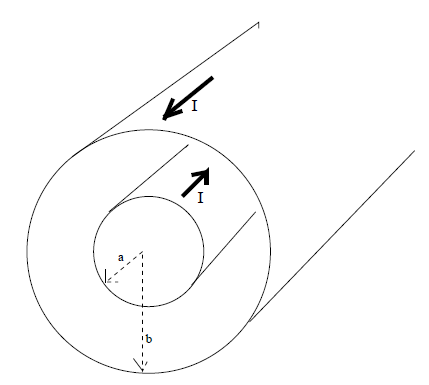
\includegraphics[scale=0.7]{eletromag-img/coaxial2.png}
%\caption{Espira que gira em torno de $z$.}
\end{figure}

\resposta


\item Uma onda plana uniforme incide, do vácuo, em uma placa de vidro que possui índice de refração $n_{2}=1,5$. O campo elétrico desta onda é:
$$
\vec{E}_{i} = 4 \operatorname{cos} \left( 4,0 \pi  \times 10^{6} z - 1,2 \times 10^{15} t   \right)\hat{e}_{x}
$$
onde todas as grandezas são expressas no SI. As trajetórias dos raios luminosos correspondentes (incidente, refletido e transmitido) são mostradas na figura a baixo.
\begin{figure}[H]
\centering
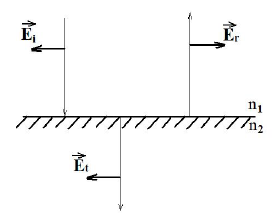
\includegraphics[scale=0.7]{eletromag-img/vidro.png}
%\caption{Espira que gira em torno de $z$.}
\end{figure}

a) Transcreva a figura no seu caderno de resposta e, para cada onda, desenhe o campo magnético $\vec{B}$ e o vetor de onda $\vec{k}$ correspondentes (preocupe-se apenas com a direção e sentido dos vetores).

\resposta

b) Determine a velocidade de propagação, o comprimento de onda e a frequência das ondas incidente, refletida e transmitida.

\resposta

c) A partir de uma das equações de Maxwell determine o campo magnético da onda incidente e também o vetor de Poynting correspondente.

\resposta


\item Considere um capacitor plano, de placas paralelas muito grandes, no vácuo, com densidades de carga $+\sigma$ e $-\sigma$, que encontra-se em repouso no referencial do laboratório.

\begin{figure}[H]
\centering
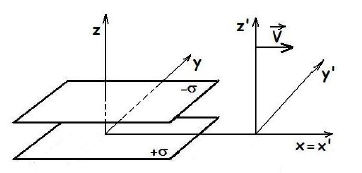
\includegraphics[scale=0.7]{eletromag-img/placas2.png}
%\caption{Espira que gira em torno de $z$.}
\end{figure}

a) Qual é o campo elétrico e o campo magnético no interior do capacitor, medidos por um observador que encontra-se no referencial do laboratório (em repouso em relação ao capacitor)?

\resposta

b) Calcule os vetores campo elétrico e magnético no interior do capacitor, medidos por um observador que encontra-se em um referencial $S'$ (ver figura acima), movendo-se ao longo do eixo $x$ com velocidade $V$ constante.

\resposta

c) Supondo agora o observador movendo-se ao longo do eixo $z$ (perpendicularmente aos planos das placas), com velocidade constante $V$, calcule novamente os vetores campo elétrico e magnético no interior do capacitor.

\resposta


\item Em uma experiência de laboratório um estudante, para determinar a constante de tempo $\tau = RC$ de um capacitor comercial $C = 1,0 \mu F$, montou o circuito da figura abaixo, utilizando um resistor de 10 $M \Omega$ e uma pilha de $1,5 \ V$. Assim, quando a chave $S_{1}$ é fechada e a $S_{2}$ aberta, o capacitor é carregado até a máxima tensão. Em $t = 0 \ s$, a chave $S_{1}$ é aberta e a $S_{2}$ é fechada, descarregando o capacitor.
\begin{figure}[H]
\centering
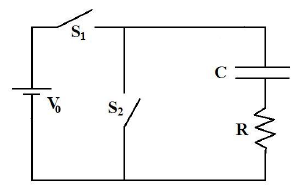
\includegraphics[scale=0.7]{eletromag-img/circuito.png}
%\caption{Espira que gira em torno de $z$.}
\end{figure}

a) Para o processo de descarga, encontre a equação do circuito, resolvendo-a em $Q$, e mostre que $V = V_{0} \operatorname{exp}(-t/RC)$ corresponde à expressão que fornece a tensão no capacitor em função do tempo.

\resposta

b) Para realizar a medida de $\tau = RC$ o estudante optou por medir o tempo ($t_{1/2}$) que leva para que a tensão no capacitor seja exatamente a metade da tensão inicial. Para isto, ele utilizou um multímetro e um cronômetro manual. O procedimento foi realizado 10 vezes e os resultados estão representados na tabela abaixo.

\begin{tabular}{|c|c|c|c|c|c|c|c|c|c|c|}
\hline
% after \\: \hline or \cline{col1-col2} \cline{col3-col4} ...
$t_{1/2} \ (s)$ & 8,12 & 8,12 & 8,15 & 8,11 & 8,13 & 8,14 & 8,13 & 8,15 & 8,12 & 8,14 \\
\hline
\end{tabular}

\noindent Após calcular o valor médio utilizando uma calculadora, o estudante escreveu em seu relatório que $\langle t_{1/2} \rangle = 8,131 \pm 0,0137 \ s$. Você concorda com a forma com que ele expressou o valor o valor médio de $t_{1/2}$? Justifique. Se não concorda, como você expressaria o valor do tempo médio medido da maneira correta?

\resposta

c) A partir do valor arredondado de $t_{1/2} = 8 \ s$ (para uma rápida avaliação dos resultados), determine o valor experimental da constante de tempo $\tau_{exp}$ e compare com o seu valor nominal $\tau_{nominal}$.

\resposta

d) Construa um gráfico da tensão (eixo $y$) em função do tempo (eixo $x$) que represente a descarga do capacitor. Mostre neste gráfico, de uma maneira aproximada, os dados mais representativos da experiência ($V_{0}, \tau, t_{1/2}$).

\resposta



\item Considere uma distribuição esférica cargas, com densidade volumétrica de cargas constante, de raio $R_{e}$ e carga total $e$.

a) Determine o vetor campo elétrico $\vec{E}$ em todo o espaço (dentro e fora da distribuição esférica).

\resposta

b) Calcule a energia total associada a esta distribuição de cargas e mostre que:
$$
U = \frac{3}{5} \frac{e^{2}}{4 \pi \epsilon_{0} R_{e}}.
$$

\resposta

c) Supor que a energia calculada no ítem anterior corresponde à massa ($m_{e}$) de repouso do elétron. Calcule a expressão que fornece o raio do elétron e faça uma estimativa do seu valor, em metros.

\resposta



\item Considere um fio reto e infinito, pelo qual flui uma corrente $I$ constante. Calcule o vetor campo magnético $\vec{B}$ em um ponto $P$, à distância $\rho$ do fio:
\begin{figure}[H]
\centering
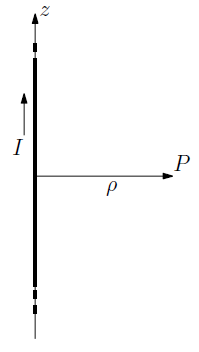
\includegraphics[scale=0.7]{eletromag-img/fio3.png}
%\caption{Espira que gira em torno de $z$.}
\end{figure}

a) utilizando a lei de Ampère:
$$
\oint \vec{B} \cdot d \vec{\ell} = \mu_{0} I;
$$

\resposta

b) utilizando a lei de Biot-Savart:
$$
d \vec{B} = \frac{\mu_{0} I}{4 \pi} \frac{d \vec{\ell} \times \hat{e}_{r}}{r^{2}}
$$

\resposta

c) através do cálculo do potencial vetor:
$$
\vec{A} =  \frac{\mu_{0}}{4 \pi} \int \frac{\vec{J} dV}{r}
$$
\item[  ] Lembre-se que $ \vec{J} dV \longleftrightarrow I d \vec{\ell} $.
\item[  ] Sugestão: Suponha um fio de comprimento $L$ muito grande, de forma que $L >> \rho$.

\resposta



\item Foi idealizado um experimento para o estudo da polarização de ondas eletromagnéticas por reflexão em uma superfície dielétrica plana. Uma onda não polarizada pode ser considerada como tendo componentes do campo elétrico paralela (componente $p$) e não paralela (componente $s$) à superfície do dielétrico, de forma que os coeficientes de Fresnel correspondentes são:
\begin{multicols}{2}
$$
r_{12p} = \frac{n_{1} \operatorname{cos} \theta_{1} - n_{2} \operatorname{cos} \theta_{2}}{n_{1} \operatorname{cos} \theta_{1} + n_{2} \operatorname{cos} \theta_{2}} = \frac{\operatorname{sen}( \theta_{2} - \theta_{1} )}{\operatorname{sen}( \theta_{2} - \theta_{1} )}; \\
$$

$$
r_{12p} = \frac{n_{1} \operatorname{cos} \theta_{1} - n_{2} \operatorname{cos} \theta_{2}}{n_{1} \operatorname{cos} \theta_{1} + n_{2} \operatorname{cos} \theta_{2}} =  \frac{\operatorname{tg}( \theta_{2} - \theta_{1} )}{\operatorname{tg}( \theta_{2} + \theta_{1} )}.\\
$$

\begin{figure}[H]
\centering
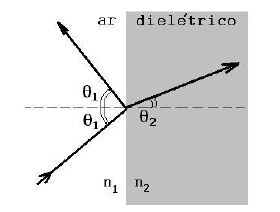
\includegraphics[scale=0.7]{eletromag-img/dieletrico2.png}
\end{figure}

\end{multicols}


a) Notando que a polarização ocorre quando $\theta_{1}$ ($\theta_{1} = \theta_{B}$) satisfaz a condição $\theta_{1} + \theta_{2} = \pi/2$, mostre que $\operatorname{tg} \theta_{B} = n_{2}/n_{1}$ e que, nesta condição, o coeficiente de Fresnel da componente da onda que não se anula pode ser escrito como:
$$
r_{12} = \frac{1 - n_{2}^{2}}{1 + n_{2}^{2}}.
$$

\resposta

b) No experimento, um painel de polietileno e um conjunto emissor/receptor de micro-ondas foi utilizado, conforme mostrado na figura a baixo.
\begin{figure}[H]
\centering
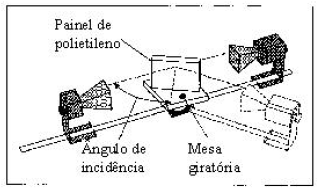
\includegraphics[scale=0.7]{eletromag-img/experimento.png}
\end{figure}
O ângulo de incidência foi sendo variado e as intensidades relativas $I_{p}/I_{0}$ e $I_{s}/I_{0}$ da onda correspondentes às componentes $p$ e $s$, foram registradas na tabela abaixo.

\begin{tabular}{|c|c|c|}
\hline
\multirow{2}{*}{Ângulo $(\theta_{1})$}
& \multicolumn{2}{c|}{Leituras dos medidores}   \\ \cline{2-3}
& $I_{s}/I_{0}$   & $I_{p}/I_{0} $              \\ \hline
20°              & $0,41 \pm 0,04$ & $0,36 \pm 0,04$             \\
25°              & $0,28 \pm 0,04$ & $0,34 \pm 0,04$             \\
30°              & $0,26 \pm 0,04$ & $0,28 \pm 0,04$             \\
35°              & $0,24 \pm 0,04$ & $0,21 \pm 0,04$             \\
40°              & $0,15 \pm 0,04$ & $0,19 \pm 0,04$             \\
45°              & $0,11 \pm 0,04$ & $0,20 \pm 0,04$             \\
\hline
\end{tabular}
\begin{tabular}{|c|c|c|}
\hline
\multirow{2}{*}{Ângulo $(\theta_{1})$}
& \multicolumn{2}{c|}{Leituras dos medidores}   \\ \cline{2-3}
& $I_{s}/I_{0}$   & $I_{p}/I_{0} $              \\ \hline
50°              & $0,10 \pm 0,04$ & $0,17 \pm 0,04$             \\
55°              & $0,05 \pm 0,04$ & $0,14 \pm 0,04$             \\
60°              & $0,03 \pm 0,04$ & $0,19 \pm 0,04$             \\
65°              & $0,04 \pm 0,04$ & $0,23 \pm 0,04$             \\
70°              & $0,19 \pm 0,04$ & $0,48 \pm 0,04$             \\
75°              & $0,44 \pm 0,04$ & $0,65 \pm 0,04$             \\
\hline
\end{tabular}

\item [  ]Com os dados da tabela construa o gráfico adequado e, a partir deste, determine o ângulo de Brewster $\theta_{B}$.

\resposta

c) Determine o índice de refração do painel de polietileno utilizado no experimento. Calcule a refletância $R$ da onda quando o ângulo de incidência da onda corresponde ao ângulo de Brewster e compare com o valor experimental.

\resposta

d) Como você relaciona este fenômeno de polarização com a utilização de óculos específicos por pessoas que vão à praia, que esquiam na neve, etc? Explique!

\resposta


\item Um cilindro muito longo de raio $R$ é fabricado com um material isolante cuja constante dielétrica é $K (= \epsilon / \epsilon_{0})$ e que possui uma densidade de carga livre cilindricamente simétrica, mas não uniforme $\rho(r)$.

a) Determine $\rho(r)$ tal que o campo elétrico dentro do cilindro seja radial apontando para fora do mesmo e com módulo constante $E_{0}$;

\resposta Usando como superfície um cilindro concêntrico de raio $r$ tal que este seja menor que $R$ e altura $h$, temos, pela lei de Gauss, ignorando o caráter finito do cilindro:
$$
\oint \vec{E} (\vec{r}) \cdot d \vec{S} = \frac{q_{int}}{e}
$$
utilizando $d\vec{S} = d A \hat{r}$, logo:
$$
\begin{array}{ccl}
  2 \pi r h |\vec{E}(\vec{r})| & = & \frac{1}{K \epsilon_{0}} \int_{0}^{r} \int_{0}^{h} \int_{0}^{2\pi} \rho (r') d^{3} r' \\
  & = & \frac{1}{K \epsilon_{0}} \int_{0}^{r} \int_{0}^{h} \int_{0}^{2\pi} \rho (r') r' d \theta' d z' d r' = \frac{2\pi h}{K \epsilon_{0}} \int_{0}^{r} \rho (r')r' d r' \\
  |\vec{E}(\vec{r})|  & = & \frac{1}{K \epsilon_{0} r} \int_{0}^{r} \rho(r') r' d r'
\end{array}
$$
Como desejamos que $\rho (\vec{r'}) = |\vec{E}| = E_{0}$, $\forall \ \epsilon \ [0, R]$, temos:
$$
|\vec{E}(\vec{r})| = E_{0} = \frac{1}{K \epsilon_{0} r} \int_{0}^{r} \rho (r') dr' \ \Rightarrow \ E_{0} K \epsilon_{0} r = \alpha r = \int_{0}^{r} \rho (r') r' dr'
$$
Sabemos que:
$$
\int_{0}^{r} \alpha d r' = \left. \alpha r' \right|_{0}^{r} = \alpha r
$$
Logo:
$$
 \rho (r') r' = \alpha \ \Rightarrow \ \rho (r') = \frac{\alpha}{r'} = \frac{E_{0} K \epsilon_{0}}{r'}
$$


b) para a densidade de carga determinada em (a), calcule o campo elétrico $\vec{E}(r)$ fora do cilindro;

\resposta Como a carga interna é:
$$
q_{int} = \int_{0}^{R} \int_{0}^{h} \int_{0}^{2\pi} \rho (r) r d \theta d z d r = 2 \pi h \int_{0}^{R} E_{0} K \epsilon_{0} d r' = \left.  2 \pi h E_{0} K \epsilon_{0} r \right|_{0}^{R} = 2 \pi h E_{0} K \epsilon_{0} R
$$
Usando como superfície um cilindro concêntrico de raio $r$ tal que este seja maior que $R$ e altura $h$, temos, pela lei de Gauss:
$$
\oint \vec{E} \vec{r} \cdot d \vec{S} = \frac{q_{int}}{\epsilon_{0}}
$$
Logo:
$$
\oint \vec{E} (\vec{r}) \cdot d \vec{S} = \frac{q_{int}}{\epsilon_{0}} \ \Rightarrow \ 2\pi h E_{0} K R = 2 \pi r h |\vec{E}(\vec{r})|
$$
Portanto, usando a simetria (adotando o sinal positivo  para a cargas positivas), sendo $\hat{r}$ o versor radial do cilindro, que aponta para fora deste:
$$
|\vec{E}(\vec{r})| = \frac{E_{0} K R}{r} \ \Rightarrow \ \vec{E}(\vec{r}) = \frac{E_{0} K R}{r} \hat{r}
$$



c) se o cilindro for então envolvido por uma casca cilíndrica condutora neutra de raio interno $a$ ($a > R$) e raio externo $b$ ($b > a$), concêtrica ao mesmo, determine as densidades de carga induzidas nas superfícies da casca condutora;

\resposta

Como os metais são condutores, o campo elétrico dentro deles deve ser nulo. Logo, ao efetuar uma lei de Gauss no interior do metal, sabemos que $\forall \ r \epsilon (a,b)$ deve valer:
$$
\oint \vec{E} \vec{r} \cdot d \vec{S} = 0 = \frac{q_{int}}{\epsilon_{0}} \Rightarrow q_{int} = 0
$$
Para que isso ocorra só há uma alternativa: deve haver uma carga de valor na superfície interna do metal, distribuída uniformemente ao longo da superfície interna do cilindro. Supondo que o metal seja eletricamente neutro, se efetuarmos outra lei de Gauss para $r > b$, notamos que a superfície externa do metal deve possuir carga $q_{int}$ também uniformemente distribuída, na superfície externa do cilindro. As densidades de carga serão, se for a altura do cilindro, com
$$
\lambda = \frac{q_{int}}{h}, \ \ \sigma_{a} = \frac{\lambda}{2 \pi a} \ \mbox{ e } \   \sigma_{b} = \frac{\lambda}{2 \pi b}.
$$


\item[] Se por densidade de carga entendermos densidade linear de carga, a superfície interna possui densidade de carga $-\lambda$ e a superfície externa possui densidade de carga $\lambda$.



\item[] Se por densidade de carga entendermos densidade superficial de carga, a superfície interna possui densidade de carga $-\sigma_{a}$ e a superfície externa possui densidade de carga $\sigma_{b}$.



d) para a situação do item (c), esboce um gráfico do módulo do campo elétrico $E(r)$ em função da distância ao eixo do cilindro, em todo o espaço.

\resposta

\begin{figure}[H]
\centering
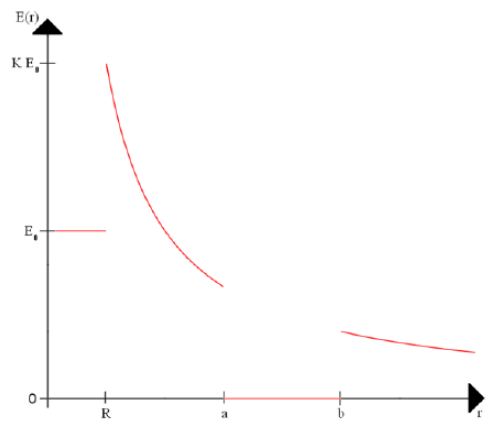
\includegraphics[scale=0.7]{eletromag-img/campo.png}
\caption{Note que o gráfico é descontínuo devido às mudanças de meios (dielétrico 1 - dielétrico 2 - metal - dielétrico 2). Note que o campo dentro do metal é nulo, e dentro do dielétrico 1 é menor devido ao maior efeito de polarizabilidade das moléculas nesta região.}
\end{figure}



\item Uma barra metálica uniforme de massa $M$ pode deslizar com atrito desprezível ao longo de um par de trilhos horizontais fixos separados por uma distância $d$, conforme mostra a figura abaixo.

\begin{figure}[H]
\centering
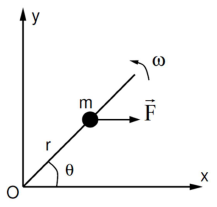
\includegraphics[scale=0.7]{eletromag-img/barra.png}
\end{figure}

Os trilhos e a ligação transversal da esquerda são altamente condutores, de modo que suas contribuições para a resistência elétrica do circuito retangular são desprezíveis. A barra livre e os contatos com os trilhos fixos têm resistência elétrica total $R$. Há um campo magnético uniforme e estacionário aplicado externamente, de módulo $B$, orientado verticalmente e apontando para cima.

a) Determine a corrente $i$ induzida no circuito em termos de $d$, $R$, $B$ e $v$, a velocidade instantânea da barra. Considere como o sentido positivo da corrente na barra aquele indicado na figura. Ao determinar a corrente induzida, despreze o campo magnético produzido pela própria corrente;

\resposta

b) suponha que em $t = 0$ a barra esteja numa posição $x_{o}$ e com velocidade $v_{o}$. Determine $x(t)$ e $v(t)$;

\resposta

c) obtenha expressões numéricas para $x(t)$, $v(t)$ e $i(t)$ usando os seguintes parâmetros: $M = 0,10 kg$, $d = 1,0  m$, $R = 1,0 \Omega$, $B = 0,2 T$, $x_{0} = 3,0 m$ e $v_{0} = 10 m/s$. Qual a posição final da barra quando ela estiver em repouso?

\resposta

d) É justificável desprezar no item (a) o campo magnético produzido pela corrente induzida? Para responder esse item, calcule a razão entre o maior valor do campo magnético produzido pela corrente induzida ($B_{i}$) e o valor do campo aplicado ($B$). Estime $B_{i}$ calculando o campo magnético na superfície da barra livre, assumindo que ela é muito longa e tem seção transversal circular com raio $a = 3,0 mm$.

\resposta


\item No instante inicial $t = 0$, uma partícula de massa $m$ e carga $q$ encontra-se na posição $x_{0} \hat{x}$ e com velocidade $v_{0} \hat{y}$. Os campos de força agindo sobre a partícula são devidos somente ao potencial elétrico $\phi$ e ao potencial vetor $\vec{A}$, dados por
$$ \Phi (\vec{r}) = \alpha_{0} x + a \alpha_{1} ; $$
$$ \vec{A} (\vec{r}) = \frac{\beta_{0}}{2} ( \vec{z} \times \vec{r} ) +  a \beta_{1} \hat{u} e^{\hat{u} \cdot \vec{r} / a} ,$$
onde $\alpha_{0}$, $\alpha_{1}$, $a$, $\beta_{0}$ e $\beta_{1}$ são constantes reais e $\hat{u}$ é um versor constante e real.

a) Calcule o vetor campo elétrico em todo o espaço, $\vec{E}(\vec{r})$.

\resposta

b) Determine o vetor indução magnética em todo o espaço, $\vec{B}(\vec{r})$.

\resposta

c) Existe algum valor para a velocidade inicial $v_{0}$ tal que a trajetória da partícula seja uma reta? Em caso afirmativo, calcule-o.

\resposta



\item Durante uma tempestade, uma nuvem cobre a cidade de São Paulo a uma altura $h = 500 m$ em relação ao solo. Vamos supor que a largura da nuvem seja bem maior que essa altura $h$. Um balão meteorológico equipado com um sensor de campo elétrico é então lançado verticalmente a partir do solo. Os dados coletados pelo sensor estão ilustrados na figura abaixo, onde $E(z)$ é o módulo do campo elétrico em função da altitude ($z = 0$ no solo). A espessura da nuvem na direção vertical é igual a $1200 m$ e sabe-se que a densidade de carga elétrica é sempre negativa no seu interior.

\begin{figure}[H]
\centering
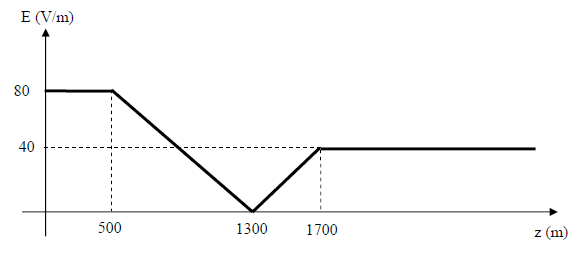
\includegraphics[scale=0.7]{eletromag-img/magnetico.png}
\end{figure}

a) Indique, em um diagrama, a direção e sentido do campo elétrico nas regiões abaixo, dentro e acima da nuvem.

\resposta

b) Calcule a densidade volumétrica de carga na atmosfera em função da altitude, $\rho(z)$, e esboce o seu gráfico.

\item[] Para quais valores de $z$ o potencial elétrico é máximo ou mínimo? Calcule o potencial elétrico nesses pontos? Tome $V = 0$ no solo.





\item Uma onda eletromagnética monocromática polarizada linearmente propagando-se ao longo da direção $+ \hat{x}$ é representada na notação complexa pelo campo elétrico $ \vec{E}(x,t) = \hat{y} E_{0} e^{i(kx - wt)} $. Considere que essa onda propaga-se no ar ($n_{ar} \approx 1$) e possui comprimento de onda $\lambda_{0} = 0,50 \mu m$ (luz verde) e intensidade $I_{0} = 10 W/m^{2}$.

a) Escreva uma expressão análoga à equação acima para o campo magnético $\vec{B}(x,t)$ dessa onda, escrevendo sua amplitude $B_{0}$ em função de $E_{0}$ no sistema SI de unidades.

\resposta

b) Essa onda incide perpendicularmente a uma placa de 1,0 $mm$ de espessura feita de um material que possui índice de refração $n = n_{R} + i n_{j}$, onde $n_{j} << n_{R}$ para ondas dessa frequência. Dada a expressão abaixo para a refletividade $R$ da interface entre o meio 1 (índice de refração $n_{1}$) e o meio 2 (índice de refração $n_{2}$), estime a partir do seguinte gráfico (intensidade I versus posição $x$) a parte real $n_{R}$ do índice de refração do material.

\resposta

c) Estime, também a partir do gráfico, a parte imaginária $n_{I}$ do índice de refração.

\resposta

d) Qual a frequência e o comprimento de onda da radiação dentro do material?

$$
R = \left| \frac{n_{1} - n_{2}}{n_{1} + n_{2}}   \right|^{2}
$$
\begin{figure}[H]
\centering
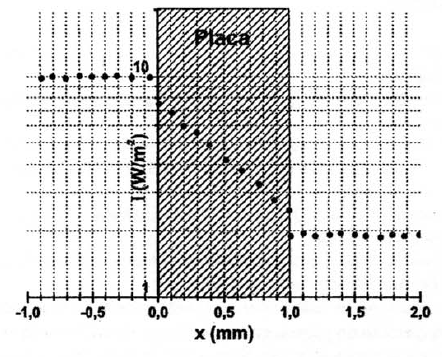
\includegraphics[scale=0.7]{eletromag-img/placa3.png}
\end{figure}

\resposta


\item Um solenoide circular é projetado com $81\pi \ mm^{2}$ de área de seção transversal e $40 \pi \ mm$ de comprimento. Desprezando os efeitos do comprimento finito do solenóide, responda:

a) Quantas voltas de fio são necessárias para que o módulo do campo magnético próximo ao centro do solenóide seja de 2,0 $mT$ quando percorrido por uma corrente de 1,0 $A$?

\resposta

b) Se o solenoide é enrolado compactamente (sem espaçamento entre voltas consecutivas) com uma única camada de fio de cobre de resistividade $2,0 \times 10^{-8} \ \Omega m$, qual é a resistência elétrica do solenoide? Despreze a espessura do isolante que recobre o fio.

\resposta

c) Que diferença de potencial deve ser aplicada nos terminais do solenóide para produzir o campo magnético de 2,0 $mT$?

\resposta

d) Para esse valor do campo, qual a energia magnética armazenada no solenoide?

\resposta

e) Determine a indutância desse solenóide.

\resposta



\item Uma placa metálica fina e carregada está imersa em uma solução aquosa de cloreto de sódio (sal de cozinha), cuja constante dielétrica é $K = \epsilon / \epsilon_{0} = 80$. Considere esta placa como infinita e situada no plano $xy$ de um sistema de coordenadas. Determinou-se que o potencial elétrico na solução nas vizinhanças da placa e dado pela seguinte expressão:
$$
V(x,y,z) = 10 \mathrm{exp}(-20|z|)
$$
com $z$ medido em metros e $V$ em volts.

a) Determine o vetor camp o elétrico correspondente a esse potencial.

\resposta

b) Qual a magnitude e sinal da densidade superficial de carga livre $\sigma(x,y)$ da placa?

\resposta

c) Determine a densidade volumétrica de carga livre $\rho(x,y,z)$ na solução, nas proximidades da placa.

\resposta


\item  O fio retilíneo muito longo da figura abaixo conduz uma corrente $i$ no sentido indicado, cuja magnitude está crescendo a uma taxa $\mathrm{d} i/\mathrm{dt}$.

a) Quando a corrente no fio é igual a $i$, calcule o fluxo magnético através da espira retangular.

\resposta

b) Obtenha uma expressão para a força eletromotriz induzida na espira.

\resposta

c) Se a resistência da espira é 0,051 $\Omega$, calcule o valor numérico da corrente induzida na espira e indique seu sentido para $a = 12 cm$, $b = 36 cm$, $L = 24 cm$ e$\mathrm{d} i/\mathrm{dt} = 9,6 \ A/s$.

\begin{figure}[H]
\centering
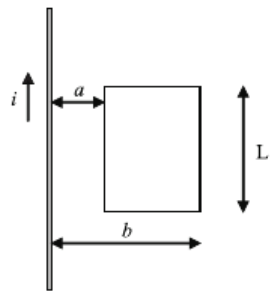
\includegraphics[scale=0.7]{eletromag-img/barrae.png}
\end{figure}

\resposta




\end{enumerate}






